\chapter{The Material Point Method} \label{ch:MPMTheory}

\section{Introduction}
The \MPM component solves the momentum equations
\Beq \label{eq:mom_mpm}
  \Div{\Bsig} + \rho\Bb = \rho\dot{\Bv} 
\Eeq
using an updated Lagrangian formulation. The momentum solve for solid materials is
complicated by the fact that the equations need material constitutive models for
closure.  These material constitutive models vary significantly between materials
and contribute a large fraction of the computational cost of a simulation.

The material point method (MPM) was described by Sulsky et al.~\cite{Sulsky1994,Sulsky1995} as
an extension to the FLIP (Fluid-Implicit Particle) method of
Brackbill~\cite{brackbill-ruppel86}, which itself is an
extension of the particle-in-cell (PIC) method of
Harlow~\cite{harlow1963}.
\begin{NoteBox}
Interestingly, the name ``material point method"
first appeared in the literature two years later in a description of
an axisymmetric form of the method~\cite{sulsky_axisym_1996}.
\end{NoteBox}
In both FLIP and \MPM, the basic idea is the same: objects are discretized into
particles, or material points, each of which contains all state data for the
small region of material that it represents.  Particles do not interact
with each other directly, rather the particle information is accumulated
to a background grid, where the equations of motion~\eqref{eq:mom_mpm} are
integrated forward in time. This time advanced solution is then used to update
the particle state.  Particle state data includes the position, mass, volume,
velocity, stress, state of deformation of that material, and a number of
time-dependent internal material variables.
\begin{NoteBox}
\MPM differs from other ``mesh-free'' particle methods in that, while each object
is primarily represented by a collection of particles, a computational mesh
is also an important part of the calculation.  This mesh reduces the computational
cost of searching for neighboring particles.
\end{NoteBox}

\MPM usually uses a regular structured grid as a computational mesh.
While this grid, in principle, deforms as the material that it is representing
deforms, at the end of each timestep, it is reset to its original undeformed
position, in effect providing a new computational grid for each timestep.
The use of a regular structured grid for each time step has a number of
computational advantages.  Computation of spatial gradients is simplified.
Mesh entanglement, which can plague fully Lagrangian techniques, such as
the Finite Element Method (FEM), is avoided.

\MPM has also been successful
in solving problems involving contact between colliding objects, having an
advantage over FEM in that the use of the regular grid eliminates the
need for doing costly searches for contact surfaces\cite{Bard2000}.

In addition to the advantages that \MPM brings, as with any numerical technique, it has
its own set of shortcomings.  It is computationally more
expensive than a comparable FEM code.  Accuracy for \MPM is typically lower
than FEM, and errors associated with particles moving around the computational
grid can introduce non-physical oscillations into the solution.  Finally,
numerical difficulties can still arise in simulations involving large
deformation that will prematurely terminate the simulation.  The severity of
all of these issues (except for the expense) has been significantly reduced
with the introduction of the Generalized Interpolation Material Point Method,
or \GIMP\cite{Bard2004}. Newer developments such as the \CPDI \MPM
method~\cite{Sadeghirad2011} have also been incorporated into the explicit
time integrated \MPM in \Vaango.  Implementation of other approaches along the
line of \CPDI such as \Textsfc{CPDI2}~\cite{Sadeghirad2013} and \Textsfc{CPTI}~\cite{Leavy2019} is
also being considered for future versions.

In addition, \MPM can be incorporated with a multi-material CFD algorithm
as the structural component in a fluid-structure interaction formulation.
This capability was first demonstrated in the CFDLIB codes from
Los Alamos by Bryan Kashiwa and co-workers\cite{Kashiwa2000}.  There, as
in the \MPMICE component, \MPM serves as the Lagrangian description of the solid
material in a multimaterial CFD code.  Certain elements of the
solution procedure are based in the Eulerian CFD algorithm, including
intermaterial heat and momentum transfer as well as satisfaction
of a multimaterial equation of state.  The use of a Lagrangian method
such as \MPM to advance the solution of the solid material eliminates
the diffusion typically associated with Eulerian methods.  

\section{Weak form of the momentum equation} \label{sec:weak_form}
To derive the weak form of the momentum equation~\eqref{eq:mom_mpm}, we multiply the 
momentum equation with a vector-valued weighting function ($\Bw$) and
integrate over the domain ($\Omega$).  The weighting function ($\Bw$)
satisfies velocity boundary conditions on the parts of the boundary
where velocities are prescribed.  Then,
\Beq
  \IntOmega \Bdot{\Bw}
                 {\LBs\Div{\Bsig} + \rho~\Bb\RBs}~d\Omega 
     = \IntOmega \rho~\Bdot{\Bw}{\dot{\Bv}}~d\Omega ~.
\Eeq
Using the identity 
$\Bdot{\Bv}{(\Div{\BS)}} = \Div{(\Bdot{\BS^T}{\Bv})} - \BS:\Grad{\Bv}$, 
where $\BS$ is a second-order tensor valued field and $\Bv$ is a 
vector valued field, we have
\begin{equation*}
  \IntOmega \LBc
     \Div{(\Bdot{\Bsig^T}{\Bw})} - \Bsig:\Grad{\Bw} +
     \rho~\Bdot{\Bw}{\Bb}\RBc~d\Omega 
     = \IntOmega \rho~\Bdot{\Bw}{\dot{\Bv}}~d\Omega \,.
\end{equation*}
Application the divergence theorem to the divergence of the weighted stress leads to
\begin{equation*}
  \IntGamma \Bdot{\Bn}{(\Bdot{\Bsig^T}{\Bw})} ~d\Gamma + 
  \IntOmega \LBc - \Bsig:\Grad{\Bw} + \rho~\Bdot{\Bw}{\Bb}\RBc~d\Omega 
     = \IntOmega \rho~\Bdot{\Bw}{\dot{\Bv}}~d\Omega  
\end{equation*}
where $\Bn$ is the outward normal to the surface $\Gamma$.  Rearranging,
\Beq
  \IntGamma (\Bsig\cdot\Bn)\cdot\Bw ~d\Gamma  
  - \IntOmega \Bsig:\Grad{\Bw}~d\Omega  
  + \IntOmega \rho~\Bdot{\Bw}{\Bb}~d\Omega
  = \IntOmega \rho~\Bdot{\Bw}{\dot{\Bv}}~d\Omega  \,.
\Eeq
If the applied surface traction is $\Bart := \Bdot{\Bsig}{\Bn}$, 
since $\Bw$ is zero on the part of the boundary where velocities/displacements
are specified, we get the \Textsfc{weak form}
\begin{NoteBox}
\Beq \label{eq:weak_form}
  \IntGammat \Bart\cdot\Bw ~d\Gamma  
  - \IntOmega \Bsig:\Grad{\Bw}~d\Omega  
  + \IntOmega \rho~\Bdot{\Bw}{\Bb}~d\Omega
  = \IntOmega \rho~\Bdot{\Bw}{\dot{\Bv}}~d\Omega  \,.
\Eeq
\end{NoteBox}

\section{Information transfer from particles to grid and back} \label{sec:projection}
The goal of \MPM is to find a unique function $f(\Bx,t)$ that satisfies the governing
equations~\eqref{eq:mom_mpm} for a given initial set of objects and a set of initial
and boundary conditions.

An important underlying assumption in \MPM is that
continuum field quantities have two equivalent representations -- a grid representation and
a particle representation.  For instance, the representation of a vector field $\Bf$ can be both 
\Beq \label{eq:mpm_rep}
  \boxed{
    \Bf(\Bx) = \sum_g \Bf(\Bx_g) S_g(\Bx) = \sum_g \Bf_g S_g(\Bx)
   }
    \quad \Tand \quad
  \boxed{
  \Bf(\Bx) = \sum_p \Bf(\Bx_p) \chi_p(\Bx) = \sum_p \Bf_p \chi_p(\Bx)
  }
\Eeq
where the subscript $g$ indicates a grid nodal quantity and the subscript $p$ indicates a
particle quantity.  A particle centroid is at the location $\Bx_p$ while a grid node is
at $\Bx_g$.  The functions $S_g$ are interpolation functions (also called shape functions)
that take values from the grid nodes to points in the computational domain.  On the
other hand, the functions $\chi_p$ are particle characteristic functions.  We assume that
both these representations are partitions of unity.  In the above we have ignored time-dependence
for simplicity.

The \MPM algorithm is particle-centered. We start with information on particles and
then project that information to the grid nodes for the solution of~\eqref{eq:mom_mpm}.  After
the equations have been solved, the information on the grid can be interpolated back to
the particles in preparation for the next timestep. The projection operation from
particles to the grid is not as obvious as the interpolation from the grid back to particles
and requires some explanation.

Ideally we would like the two representations in \eqref{eq:mpm_rep} to produce identical
results.  However, due to approximation errors, they usually do not.  Let $\Be(\Bx)$ be the
error.  Then we can pose a least-squares error minimization problem as
\Beq
 \text{Find}~~\Bf_g~~\text{that minimizes}~~ E = \IntOmega w(\Bx)\Norm{\Be(\Bx)}{}^2\, d\Omega~~
   \text{where}~~\IntOmega w(\Bx)\,d\Omega = 1 \,. 
\Eeq
The domain of integration is the volume $\Omega$ and $w(\Bx)$ is a weighting function.
Then the minimum of the functional $E$ can be found using
\Beq
  \Partial{E}{\Bf_g} = \Bzero \quad \implies \quad
  \IntOmega w(\Bx)\left[\Partial{\Be}{\Bf_g}\cdot\Be(\Bx) + \Be(\Bx)\cdot\Partial{\Be}{\Bf_g}\right]\,d\Omega = \Bzero
\Eeq
From \eqref{eq:mpm_rep},
\Beq
  \Partial{\Be}{\Bf_g} =
    \Partial{}{\Bf_g}\left[\sum_{g'} \Bf_{g'} S_{g'}(\Bx) - \sum_p \Bf_p \chi_p(\Bx) \right]
    = \sum_{g'} \Partial{\Bf_{g'}}{\Bf_g} S_{g'}(\Bx) = S_g(\Bx)\,\BI \,.
\Eeq
Therefore,
\Beq
  \IntOmega w(\Bx) S_g(\Bx)\Be(\Bx)\,d\Omega = \Bzero
  \quad \implies \quad
  \IntOmega w(\Bx) S_g(\Bx)\left[\sum_{g'} \Bf_{g'} S_{g'}(\Bx) - \sum_p \Bf_p \chi_p(\Bx) \right]\,d\Omega = \Bzero \,.
\Eeq
If we note that the particle characteristic function ($\chi_p$) is required to be zero outside the
domain of particle $p$ and 1 inside, rearrangement of the above equation leads to
\Beq \label{eq:g_p_map_0}
  \sum_g \Bf_g \IntOmega w(\Bx) S_{g'}(\Bx) S_g(\Bx)\,d\Omega =
    \sum_p \Bf_p \IntOmegap w(\Bx) S_{g'}(\Bx)\,d\Omega \,.
\Eeq
Define
\Beq \label{eq:Sgp_def}
  \boxed{
  A_{g'g} := \IntOmega w(\Bx) S_{g'}(\Bx) S_g(\Bx)\,d\Omega
  \quad \Tand \quad
  B_{g'p} := \IntOmegap w(\Bx) S_{g'}(\Bx)\,d\Omega \,.
  }
\Eeq
Equation \eqref{eq:g_p_map_0} can now be expressed as
\Beq \label{eq:g_p_map_1}
  \sum_g A_{g'g} \Bf_g = \sum_p B_{g'p} \Bf_p \,.
\Eeq
Inverting the relation, we have
\Beq
  \Bf_g = \left[\SfA^{-1}\right]_{gg'} \sum_p B_{g'p} \Bf_p 
        = \sum_p \left[\SfA^{-1}\right]_{gg'} B_{g'p} \Bf_p 
\Eeq
where $\SfA$ is the matrix representation of $A_{g'g}$ in \eqref{eq:g_p_map_1}. We
can rewrite the above equation as
\Beq \label{eq:g_p_map}
  \boxed{
  \Bf_g = \sum_p \psi_{gp} \Bf_p 
  }
\Eeq
where
\Beq \label{eq:psi_gp}
  \boxed{
  \psi_{gp} := \left[\SfA^{-1}\right]_{gg'} B_{g'p}\,.
  }
\Eeq
\begin{NoteBox}
  The map in equation~\eqref{eq:g_p_map} can be used to project particle quantities to grid nodes.
  However, some simplification is needed to avoid the need to invert a large matrix.
\end{NoteBox}

We can remove the need to invert $\SfS$ if we diagonalize $S_{g'g}$ using a lumped approximation.
In that case
\Beq
  A_{g'} = \sum_g A_{g'g} = \IntOmega w(\Bx) S_{g'}(\Bx) \sum_g S_g(\Bx) \,d\Omega
     = \IntOmega w(\Bx) S_{g'}(\Bx) \,d\Omega
\Eeq
where we have used the partition of unity property of the grid nodal interpolation
function.  Now note that the integral over the domain $\Omega$ can be split into a sum of integrals
over particles.  

\begin{NoteBox}
The particle-to-grid projection operations in equations~\eqref{eq:g_p_map} and
\eqref{eq:psi_gp} can then be expressed as
\Beq \label{eq:particle_to_grid_gen}
  \Bf_g = \sum_p \psi_{gp} \Bf_p \quad \text{where} \quad
  \psi_{gp} = \frac{B_{gp}}{A_g}~,~~
  A_{g} = \sum_p B_{gp} ~,~~
  B_{gp} = \IntOmegap w(\Bx) S_{g}(\Bx) \,d\Omega \,.
\Eeq
\end{NoteBox}

Going back to \eqref{eq:mpm_rep}, recall that we had assumed that $\Bf_p$ was the value
of the function $\Bf(\Bx)$ at the particle centroid, $\Bx_p$.  However, this requirement
is not necessary for the development of the projection from particles to the grid.  We
may, alternatively, define $\Bf_p$ as
\Beq \label{eq:f_p}
  \Bf_p = \frac{1}{W_p} \IntOmegap \Bf(\Bx) \omega_p(\Bx)\,d\Omega ~,~~
  W_p := \IntOmegap \omega_p(\Bx)\,d\Omega
\Eeq
where $\Omega_p$ is the particle domain and $\omega_p(\Bx)$ is a weighting function.
Also recall that the grid interpolation function has the form
\Beq \label{eq:f_g}
  \Bf(\Bx) = \sum_g \Bf_g S_g(\Bx)\,.
\Eeq
Therefore, we can compute the value of a quantity at a particle using the grid interpolation
functions by substituting \eqref{eq:f_g} into \eqref{eq:f_p} to get
\Beq
  \Bf_p = \frac{1}{W_p} \IntOmegap \left[\sum_g \Bf_g S_g(\Bx)\right] \omega_p(\Bx)\,d\Omega 
        = \sum_g \Bf_g \left[\frac{1}{W_p} \IntOmegap S_g(\Bx) \omega_p(\Bx)\,d\Omega\right] \,.
\Eeq
Since the particle domain $\Omega_p$ is never known exactly and we would like to avoid
determining that domain, we approximate the above equation as
\Beq
  \Bf_p \approx \sum_g \Bf_g \left[\frac{1}{W^\star_p} \int_{\Omega_p^\star} S_g(\Bx) \omega^\star_p(\Bx)\,d\Omega\right] ~,~~
  W^\star_p := \int_{\Omega_p^\star}\omega^\star_p(\Bx)\,d\Omega
\Eeq
where the alternative weight function $\omega^\star_p(\Bx)$ is defined as
\Beq
  \omega^\star_p(\Bx) := \omega_p(\Bx) \,\chi^\star_p(\Bx)\,d\Omega \,.
\Eeq
The function $\chi^\star_p(\Bx)$ is called the \Textsfc{particle averaging function} since it is
is {\Red not} identical to the \Textsfc{particle characteristic function} $\chi_p(\Bx)$.  All
that is needed is that the function have compact support in a neighborhood
$\Omega_p^\star$ containing particle $p$.

\begin{NoteBox}
The grid-to-particle interpolation function can then be expressed as
\Beq \label{eq:grid_to_particle}
  \Bf_p \approx \sum_g \Bf_g \Av{S_{gp}} \quad\text{where}\quad
  \Av{S_{gp}} := \frac{\int_{\Omega_p^\star} S_g(\Bx) \omega^\star_p(\Bx)\,d\Omega}{
                       \int_{\Omega_p^\star} \omega^\star_p(\Bx)\,d\Omega} ~,~~
  \omega^\star_p(\Bx) := \omega_p(\Bx) \,\chi^\star_p(\Bx)\,d\Omega \,.
\Eeq
\end{NoteBox}
A more compact matrix notation is used in~\cite{Nairn2020}:
\Beq \label{eq:mat_g_to_p}
 \BfT_p = \SfS \BfT_g
\Eeq
where $\BfT_p$ is a particle-based quantity matrix that has size $N_p \times 1$ for scalars,
$N_p \times 3$ for vectors, and $N_p \times 6$ for symmetric second-order tensors. The
matrix $\BfT_g$ are the corresponding grid quantities that have sizes $N_g \times 1$ for scalars,
$N_g \times 3$ for vectors and $N_f \times 6$ for symmetric 2-tensors. The $\SfS$ matrix has
size $N_p \times N_g$ with components $\Av{S_{gp}}$.

We can now make some special assumptions about the weight functions in \eqref{eq:particle_to_grid_gen} to
reduce the projection operation to that use in tradition \MPM approaches.  Let us assume that
\Beq
  B_{gp} = V_p\Av{S_{gp}} \quad \implies \quad
  \IntOmegap S_{g}(\Bx) w(\Bx) \,d\Omega = 
  V_p\frac{\IntOmegap S_g(\Bx) \omega_p(\Bx)\,d\Omega}{\IntOmegap \omega_p(\Bx)\,d\Omega} 
\Eeq

\begin{NoteBox}
With that assumption, the particle-to-grid projection operations in equations~\eqref{eq:particle_to_grid_gen} 
become
\Beq \label{eq:particle_to_grid}
  \Bf_g = \sum_p \psi_{gp} \Bf_p \quad \text{where} \quad
  \psi_{gp} = \frac{V_p\Av{S_{gp}}}{\sum_p V_p\Av{S_{gp}}}~,~~\sum_p \psi_{gp} = 1 \,.
\Eeq
\end{NoteBox}
The matrix notation used for the above relation in~\cite{Nairn2020} is
\Beq \label{eq:mat_p_to_g}
  \BfT_g = \SfS^\plus \BfT_p
\Eeq
where $\SfS^\plus$ is a $N_g \times N_p$ matrix.

\subsection{Traditional MPM}
If we wish to recover the traditional \MPM formulation~\cite{Sulsky1995}, take $\omega_p(\Bx) = 1$
and $\chi^\star_p(\Bx) = V_p \delta(\Bx - \Bx_p)$ where $V_p$
is the volume of $\Omega^\star_p = \Omega_p$ and $\delta(\Bx)$ is the Dirac delta function, we have
\Beq
  \overbar{S}_{gp} := \Av{S_{gp}} = \frac{\int_{\Omega_p} S_g(\Bx) V_p \delta(\Bx - \Bx_p)\,d\Omega}{
                       \int_{\Omega_p} V_p \delta(\Bx - \Bx_p)\,d\Omega} = S_g(\Bx_p)\,.
\Eeq
The gradient of the interpolation function evaluated at the particle is
\Beq \label{eq:G_mpm}
  \overbar{\BGv}_{gp} = \Av{\Grad{S_{gp}}} = \frac{\int_{\Omega_p} \Grad{S_g(\Bx)} V_p \delta(\Bx - \Bx_p)\,d\Omega}{
                       \int_{\Omega_p} V_p \delta(\Bx - \Bx_p)\,d\Omega} = \Grad{S_g(\Bx_p)}\,.
\Eeq

\subsection{GIMP}
To recover the \GIMP formulation~\cite{Bard2004}, we take $\omega_p(\Bx) = 1$ and
the square pulse function $\chi^\star_p(\Bx) = 1$ for $\Bx \in \Omega_p^\star$ and
$\chi^\star_p(\Bx) = 0$ otherwise.  The particle domain $\Omega_p^\star$ is assumed to
be a rectangular parallelepiped.  Then
\Beq
  \overbar{S}_{gp} := \Av{S_{gp}} = \begin{cases}
                \frac{1}{V^\star_p} \int_{\Omega_p^\star} S_g(\Bx)\,d\Omega & \quad \text{for}~~\Bx \in \Omega_p^\star \\
                0 & \quad \text{otherwise.}
              \end{cases}
\Eeq
The gradient of the interpolation function is
\Beq \label{eq:G_gimp}
  \overbar{\BGv}_{gp} = \Av{\Grad{S_{gp}}} = \begin{cases}
                \frac{1}{V^\star_p} \int_{\Omega_p^\star} \Grad{S_g(\Bx)}\,d\Omega & \quad \text{for}~~\Bx \in \Omega_p^\star \\
                0 & \quad \text{otherwise.}
              \end{cases}
\Eeq

\subsection{CPDI}
For the \CPDI formulation~\cite{Sadeghirad2011},  we take $\omega^\star_p(\Bx) = 1$ and
the particle domain $\Omega_p^\star$ is assumed to be a general parallelepiped that
deforms based on the particle deformation gradient.  The expression for $\phi_{gp}$ is
similar to that for \GIMP except that a modified shape function is used for interpolation:
\Beq
  \overbar{S}_{gp} := \Av{S_{gp}} = \begin{cases}
                \frac{1}{V^\star_p} \int_{\Omega_p^\star} S_g^\star(\Bx)\,d\Omega & \quad \text{for}~~\Bx \in \Omega_p^\star \\
                0 & \quad \text{otherwise.}
              \end{cases}
\Eeq
The gradient of the interpolation function is
\Beq \label{eq:G_cpdi}
  \overbar{\BGv}_{gp} = \Av{\Grad{S_{gp}}} = \begin{cases}
                \frac{1}{V^\star_p} \int_{\Omega_p^\star} \Grad{S_g^\star(\Bx)}\,d\Omega & \quad \text{for}~~\Bx \in \Omega_p^\star \\
                0 & \quad \text{otherwise.}
              \end{cases}
\Eeq

\subsection{Transfer to and from grid}
For the interpolation from grid nodes to particles, the above relations indicate a
general relation (see \eqref{eq:grid_to_particle})
\Beq
  \Bf_p = \sum_g \Bf_g \overbar{S}_{gp} \,.
\Eeq
In matrix form (see \eqref{eq:mat_g_to_p})
\Beq
  \BfT_p = \SfS \BfT_g \,.
\Eeq

For the particle-to-grid projection (see \eqref{eq:particle_to_grid_gen}), consider the
case where $w(\Bx) = \rho(\Bx)$ where $\rho$ is the mass density.  Then,
\Beq
  A_g = \IntOmega \rho(\Bx) S_g(\Bx) \,d\Omega = m_g ~,~~
  B_{gp} = \IntOmega \rho(\Bx) S_g(\Bx) \chi_p(\Bx) \,d\Omega
\Eeq
and
\Beq \label{eq:mass_weighted}
  \boxed{
  m_g \Bf_g = \sum_p \Bf_p \IntOmega \rho(x) S_g(x) \chi_p(\Bx) \,d\Omega 
            = \sum_p \Bf_p m_p \bar{S}_{gp}\,.
  }
\Eeq
where $m_g$ is the grid node mass and $m_P$ is the particle mass.
In matrix form equation~\ref{eq:mass_weighted} can be written as (see \eqref{eq:mat_p_to_g})
\Beq \label{eq:mass_weighted_mat}
  \BfT_g = \SfS^\plus \BfT_p \quad \text{where} \quad
  \SfS^\plus := \BmT_g^{-1} \SfS^T \BmT_p
\Eeq
where $\BmT_g$ is a $N_g \times N_g$ diagonal matrix that is invertible as long as $m_g \ne 0$,
$\BmT_p$ is a $N_p \times N_p$ diagonal matrix, and $\SfS$ is a $N_p \times N_g$ matrix.

On the other hand, if $w(\Bx) = 1$, we have
\Beq
  A_g = \IntOmega  S_g(\Bx) \,d\Omega = V_g ~,~~
  B_{gp} = \IntOmega S_g(\Bx) \chi_p(\Bx) \,d\Omega 
\Eeq
and
\Beq \label{eq:vol_weighted}
  \boxed{
  V_g \Bf_g = \sum_p \Bf_p \IntOmega S_g(x) \chi_p(\Bx) \,d\Omega 
            = \sum_p \Bf_p V_p \bar{S}_{gp}\,.
  }
\Eeq
where $V_g$ is the grid node volume and $V_p$ is the particle volume.
In matrix form equation~\eqref{eq:vol_weighted} can be written as
\Beq \label{eq:vol_weighted_mat}
  \BfT_g = \SfS_V^\plus \BfT_p \quad \text{where} \quad
  \SfS_V^\plus := \BV_g^{-1} \SfS^T \BV_p
\Eeq
where $\BV_g$ is a $N_g \times N_g$ diagonal matrix that is invertible as long as $V_g \ne 0$,
and $\BV_p$ is a $N_p \times N_p$ diagonal matrix.

In traditional \MPM, the velocity ($\Bv$) is projected using mass weighting as
per~\eqref{eq:mass_weighted}), i.e.,
\Beq \label{eq:mass_weighted_vel}
  m_g \Bv_g = \sum_p m_p \Bv_p \bar{S}_{gp} \quad \text{or} \quad
  \BvT_g = \SfS^\plus \BvT_p \,.
\Eeq
This implies that the mass density ($\rho$) and the momentum {\em per unit volume} ($\BPv = \rho\Bv$)
are  projected to grid nodes using the volume-weighted
approach in \eqref{eq:vol_weighted}:
\Beq \label{eq:vol_weighted_mom}
  \Bal
    V_g \rho_g = \sum_p V_p \rho_p \bar{S}_{gp} \quad \text{or} \quad
    \BmT_g = \SfS^T \BmT_p \\
    V_g \BPv_g = \sum_p V_p \BPv_p \bar{S}_{gp} \quad \text{or} \quad
    \BpT_g = \SfS^T \BpT_p
  \Eal
\Eeq
where $\BpT$ is a matrix of {\em total} momentum.
Further details
of the actual projection operators used in \Vaango are discussed next.

\section{MPM discretization of the weak form} \label{sec:discretization}
The weak form of the momentum equation is
\Beq \label{eq:weak_form_1}
  \IntGammat \Bart\cdot\Bw ~d\Gamma  
  - \IntOmega \Bsig:\Grad{\Bw}~d\Omega 
  + \IntOmega \rho~\Bdot{\Bw}{\Bb}~d\Omega = 
  \IntOmega \rho~\Bdot{\Bw}{\dot{\Bv}}~d\Omega  \,.
\Eeq

To discretize the weak form we can use either of the assumed description of
field variables shown in \eqref{eq:mpm_rep}.  The grid node-based discretization
is used in finite elements while \MPM uses the particle-based discretization but
also a grid-based approximation.

Recall from \eqref{eq:mpm_rep} and \eqref{eq:particle_to_grid} that
\Beq 
  \Bf(\Bx) = \sum_g \Bf_g S_g(\Bx) \quad \Tand \quad
  \Bf_g = \sum_p \psi_{gp} \Bf_p~,~~
  \psi_{gp} = \frac{V_p\Av{S_{gp}}}{\sum_p V_p\Av{S_{gp}}}~,~~\sum_p \psi_{gp} = 1 \,.
\Eeq
Therefore, we can write
\Beq \label{eq:Yp}
  \Bf(\Bx) = \sum_g \sum_p \psi_{gp} \Bf_p S_g(\Bx) 
           = \sum_p \Bf_p \sum_g \psi_{gp} S_g(\Bx)
           = \sum_p \Bf_p Y_p(\Bx)
\Eeq
where the \Textsfc{particle basis functions}, $Y_p$, are defined as
\begin{NoteBox}
\Beq
  Y_p(\Bx) := \sum_g \psi_{gp} S_g(\Bx) = \frac{V_p \sum_g \Av{S_{gp}}S_g(\Bx)}{\sum_p V_p\Av{S_{gp}}}
\Eeq
\end{NoteBox}
If we compare \eqref{eq:Yp} with the particle representation in \eqref{eq:mpm_rep}:
\Beq
  \Bf(\Bx) = \sum_p \Bf_p \chi_p(\Bx)
\Eeq
we see that for the grid-based and particle-based representations to be both accurate
representations of the field we need the $\chi_p$ and $Y_p$ values to be related by
\Beq
  \IntOmega w(\Bx) \chi_p(\Bx) = \IntOmega w(\Bx) Y_p(\Bx)
\Eeq
because they cannot be point-wise identical unless the particle characteristic functions
satisfy the Kronecker property exactly.  We will use the $Y_p$ \Textsfc{particle basis functions}
to discretize the momentum equation.

The first step in the MPM discretization is to convert the integrals
over $\Omega$ in \eqref{eq:weak_form_1} into a sum of integrals over particles using
the particle basic functions, $Y_p$: 
\Beq \label{eq:disc_part}
  \Bal
  &\IntGammat \Bart(\Bx)\cdot\Bw(\Bx) ~d\Gamma  
  - \sum_p\IntOmegap Y_p(\Bx)\Bsig_p:\Grad{\Bw}~d\Omega 
  + \sum_p\IntOmegap Y_p(\Bx)\rho_p\Bw(\Bx)\cdot\Bb_p~d\Omega \\
  &\quad\quad = \sum_p\IntOmegap Y_p(\Bx)\rho_p\Bw(\Bx)\cdot\dot{\Bv}(\Bx)~d\Omega  \,.
  \Eal
\Eeq
The weighting function, the velocity, and the material time derivative of $\Bv$ are approximated
as (see \cite{Sulsky1995}):
\Beq
  \Bw(\Bx) = \sum_g \Bw_g S_g(\Bx) ~,~~
  \Bv(\Bx) = \sum_h \Bv_h S_h(\Bx) ~,~~
  \dot{\Bv}(\Bx) \approx \sum_h \dot{\Bv}_h S_h(\Bx) ~.
\Eeq
Plugging these into the left hand side of \eqref{eq:disc_part} we get
\Beq 
  \Bal
  \text{LHS} &= 
  \IntGammat \Bart(\Bx)\cdot\left[\sum_g \Bw_g S_g(\Bx)\right] ~d\Gamma  
  - \sum_p\IntOmegap Y_p(\Bx)\Bsig_p:\left[\sum_g \Bw_g \otimes \Grad{S_g}\right]~d\Omega \\
  &\qquad + \sum_p\IntOmegap Y_p(\Bx)\rho_p\left[\sum_g \Bw_g S_g(\Bx)\right]\cdot\Bb_p~d\Omega 
  \Eal
\Eeq
Rearranging,
\Beq 
  \Bal
  \text{LHS} = \sum_g \Bw_g \cdot & \left[
    \IntGammat \Bart(\Bx) S_g(\Bx) ~d\Gamma  
    - \sum_p\IntOmegap Y_p(\Bx)\Bsig_p \cdot \Grad{S_g}~d\Omega\right. \\
  &\qquad\left. + \sum_p\IntOmegap \rho_p Y_p(\Bx) S_g(\Bx)\Bb_p~d\Omega \right]
  \Eal
\Eeq
Similarly, the right hand side of \eqref{eq:disc_part} can be written as
\Beq
  \text{RHS} = 
  \sum_p\IntOmegap Y_p(\Bx)\rho_p\left[\sum_g \Bw_g S_g(\Bx)\right]\cdot
                                 \left[\sum_h \dot{\Bv}_h S_h(\Bx)\right]~d\Omega  \,.
\Eeq
Rearrangement leads to
\Beq
  \text{RHS} = 
  \sum_g \Bw_g \cdot \sum_h \left[\sum_p\IntOmegap \rho_p Y_p(\Bx) S_g(\Bx) S_h(\Bx)
                                  \dot{\Bv}_h~d\Omega\right]  \,.
\Eeq
Combining the left and right hand sides and invoking the arbitrariness of
$\Bw_g$, for $N_g$ grid points we get equations for $g=1,2,\dots,N_g$:
\Beq \label{eq:integral_weak_form}
  \Bal
   \IntGammat \Bart(\Bx) S_g(\Bx) ~d\Gamma  
  & - \sum_p\IntOmegap Y_p(\Bx)\Bsig_p \cdot \Grad{S_g}~d\Omega 
    + \sum_p\IntOmegap \rho_p Y_p(\Bx) S_g(\Bx)\Bb_p~d\Omega \\
  &\qquad
    = \sum_h \left[\sum_p\IntOmegap \rho_p Y_p(\Bx) S_g(\Bx) S_h(\Bx)
                                    \dot{\Bv}_h~d\Omega\right]  \,.
  \Eal
\Eeq
We can simplify the above equations further by taking the particle variables
outside the integral by assuming they are constant over a particle domain:
\Beq \label{eq:discretized}
  \Bal
   \IntGammat \Bart(\Bx) S_g(\Bx) ~d\Gamma  
  & - \sum_p \Bsig_p  \cdot  \left[\IntOmegap Y_p(\Bx)\Grad{S_g}~d\Omega\right] 
    + \sum_p \rho_p \Bb_p \left[\IntOmegap Y_p(\Bx) S_g(\Bx)~d\Omega\right] \\
  &\qquad
    = \sum_h \sum_p \rho_p \left[\IntOmegap Y_p(\Bx) S_g(\Bx) S_h(\Bx)~d\Omega\right]
                                    \dot{\Bv}_h  \,.
  \Eal
\Eeq
Recalling that $Y_p$ has the same effect as $\chi_p$ when integrated over a particle volume,
we can write
\Beq
   \Av{S_{gp}} := \frac{1}{V_p} \IntOmegap Y_p(\Bx)~S_g(\Bx)~d\Omega \,.
\Eeq
Then \eqref{eq:discretized} can be expressed as
\Beq \label{eq:discretized1}
  \Bal
   \IntGammat \Bart(\Bx) S_g(\Bx) ~d\Gamma  
  & - \sum_p V_p \Bsig_p  \cdot  \Av{\Grad{S_{gp}}} 
    + \sum_p V_p \rho_p \Bb_p \Av{S_{gp}} \\
  &\qquad
    = \sum_h \sum_p \rho_p \left[\IntOmegap Y_p(\Bx) S_g(\Bx) S_h(\Bx)~d\Omega\right]
                                    \dot{\Bv}_h  \,.
  \Eal
\Eeq
\begin{NoteBox}
Define the mass matrix ($\BM$), the internal force vector ($\Bf_g^{\Tint}$), 
the body force vector ($\Bf_g^{\Tbody}$), and the  external force vector ($\Bf_g^{\Text}$)
at grid node $g$ as
\Beq \label{eq:discretized_def}
  \Bal
   &M_{gh} := \sum_p \rho_p\IntOmegap Y_p(\Bx)~S_g(\Bx)~S_h(\Bx)~d\Omega \\
   &\Bf_g^{\Tint} := \sum_p V_p \Bsig_p \cdot \Av{\Grad{S_{gp}}} \\
   &\Bf_g^{\Tbody} := \sum_p m_p\Bb_p~\Av{S_{gp}} \\
   &\Bf_g^{\Text} := \IntGammat \Bart(\Bx)~S_g(\Bx)~d\Gamma \,.
  \Eal
\Eeq
Then, from \eqref{eq:discretized1} we get the semi-discrete system of equations
\Beq \label{eq:discrete_MPM_equations}
  \sum_h M_{gh} \dot{\Bv}_h = \Bf_g^{\Text} -\Bf_g^{\Tint} + \Bf_g^{\Tbody} 
      ~;~~ g = 1 \dots N_g
\Eeq
\end{NoteBox}
The mass matrix is typically lumped such that
\Beq
  \Bal
  m_{g} &= \sum_h M_{gh} = \sum_p \rho_p\IntOmegap Y_p(\Bx)~S_g(\Bx)~\left[\sum_h S_h(\Bx)\right]~d\Omega 
        = \sum_p \rho_p\IntOmegap Y_p(\Bx)~S_g(\Bx)~d\Omega \\
        &= \sum_p \rho_p V_p \Av{S_{gp}}  = \sum_p m_p \Av{S_{gp}} \,.
  \Eal
\Eeq
In that case the semi-discrete system of equations simplifies to
\Beq \label{eq:semialgebraic_mpm}
  m_{g} \dot{\Bv}_g = \Bf_g^{\Text} -\Bf_g^{\Tint} + \Bf_g^{\Tbody} 
      ~;~~ g = 1 \dots N_g
\Eeq
The external force at grid nodes is more difficult to estimate and is
typically computed from particle values using
\Beq
  \Bf^{\Text}_g = \sum_p \Bf^{\Text}_p \Av{S_{gp}} \,.
\Eeq

\subsection{Damping}
Two types of artificial damping are implemented in \Vaango.  The first approach modifies 
the acceleration in \eqref{eq:semialgebraic_mpm} such that
\Beq \label{eq:semialgebraic_mpm_damping}
  m_{g} \dot{\Bv}_g = \Bf_g^{\Text} -\Bf_g^{\Tint} + \Bf_g^{\Tbody} - \alpha_d \Bv_g
      ~;~~ g = 1 \dots N_g
\Eeq
where $\alpha_d$ is a damping coefficient.

The second approach uses Richtmyer-von Neumann artificial viscosity to damp out large 
oscillations in high strain-rate simulations.  \Vaango uses a three-dimensional form 
of the Richtmyer-von Neumann artificial viscosity (\cite{VonNeumann1950,Wilkins1999}, p.29).  
The viscosity factor takes the form
\begin{equation}\label{eq:artificialVisc}
  q = C_0~\rho~l~\sqrt{\frac{K}{\rho}}\left|\Tr{\BdT}\right| +
      C_1~\rho~l^2~\left(\Tr{\BdT}\right)^2
\end{equation}
where $C_0$ and $C_1$ are constants, $\rho$ is the mass density,
$K$ is the bulk modulus, $\BdT$ is the rate of deformation tensor, and
$l$ is a characteristic length (usually the grid cell size).  Typical values
of the coefficients are $C_0 = 0.2$ and $C_1 = 2.0$.

The factor $q$ is used to decrease the particle stress:
\Beq
  \Bsig_p = \Bsig_p - q \BI 
\Eeq
before it is projected to grid nodes for internal force calculations.

\section{Algorithm Description} \label{Sec:AlgDesc}
The interested reader should consult \cite{Sulsky1994,Sulsky1995} for the development
of the discrete equations in \MPM discussed in this section, and \cite{Bard2004} for
the development of the equations for the \GIMP method.  These end up being very similar,
the differences in how the two developments affect implementation will be described in
Section~\ref{gimp_mpm}.

In solving a structural mechanics problem with \MPM, one begins by discretizing
the object of interest into a suitable number of particles, or ``material
points''.
\begin{NoteBox}
  What constitutes a suitable number is something of an open
question, but it is typically advisable to use at least two particles in each
computational cell in each direction, i.e. 4 particles per cell (PPC) in 2-D,
8 PPC in 3-D.
\end{NoteBox}

In choosing the resolution of the computational grid, similar
considerations apply as for any computational method (trade-off between
time to solution and accuracy, use of resolution studies to ensure convergence
in results, etc.).)  Each of these particles will carry, minimally, the
following variables:
\begin{itemize}
\item position - $\Bx_p$
\item mass - $m_p$
\item volume - $V_p$
\item velocity - $\Bv_p$
\item stress - $\Bsig_p$ 
\item deformation gradient - $\BF_p$
\end{itemize}

The description that follows is a recipe for advancing each of these
variables from the current (discrete) time $t_n$ to the subsequent
time $t_{n+1}$.  Note that particle mass, $m_p$, typically remains constant
throughout a simulation unless solid phase reaction models are utilized,
a feature that is not present in \Vaango \MPM.  (Such models are available
in \MPMICE, see Section \ref{ch:MPMICE}.)  It is also important to point
out that the algorithm for advancing the timestep is based on the so-called
Update Stress Last (USL) algorithm.
\begin{NoteBox}
The superiority of this approach over
the Update Stress First (USF) approach was clearly demonstrated by Wallstedt
and Guilkey \cite{WallstedtJCP}.  USF was the formulation used in Uintah
until mid-2008.
\end{NoteBox}

The discrete momentum equation that results from the weak form is given as:
\Beq \label{newton2}
  \BMv \Ba = \Bf^{\Text} - \Bf^{\Tint}  + \Bf^{\Tbody}
\Eeq
where $\BMv$ is the mass matrix, $\Ba$ is the acceleration vector,
$\Bf^{\Text}$ is the external force vector (sum of the body forces and
tractions), and $\Bf^{\Tint}$ is the internal force vector resulting from
the divergence of the material stresses.  The construction of each of these
quantities, which are based at the nodes of the computational grid,
will be described below.

The solution begins by projecting the particle state to the
nodes of the computational grid, to form the mass matrix $\BMv$ and to find
the nodal external forces $\Bf^{\Text}$, and velocities,
$\Bv$.  In practice, a lumped mass matrix is used to avoid the need to
invert a system of equations to solve Eq. \eqref{newton2} for acceleration.
These quantities are calculated at individual nodes by the following equations,
where the $\sum\limits_{p}$ represents a summation over all particles:
\Beq \label{accumulate}
  m_g = \sum_p m_p \overbar{S}_{gp} ~,~~
  \Bv_g = \frac{\sum_p m_p \Bv_p \overbar{S}_{gp}}{m_g}~,~~
  \Bf^{\Text}_g = \sum_p \Bf^{\Text}_p \overbar{S}_{gp}
\Eeq
and $g$ refers to individual nodes of the grid, $m_p$ is the particle
mass, $\Bv_p$ is the particle velocity, and $\Bf^{\Text}_p$ is the
external force on the particle.  The external forces that start on the
particles typically the result of tractions, the application of which is
discussed in the \Vaango User manual.
$\overbar{S}_{gp} = \Av{S_{gp}}$ is the shape function of the $g$-th node evaluated at
the particle $p$ as discussed in the section~\ref{sec:projection} equation~\eqref{eq:grid_to_particle}.
The functional form of the shape functions differs between \MPM, \GIMP, and \CPDI.
Further details of the difference are given in Section \ref{gimp_mpm}.

Following the operations in Eq.~\ref{accumulate}, $\Bf^{\Tint}$
is still required in order to solve for acceleration at the nodes.
This is computed at the nodes as a volume integral of the divergence
of the stress on the particles, specifically:
\Beq \label{computeIntForce}  
  \Bf^{\Tint}_g = \sum_p V_p \Bsig_p \overbar{\BGv}_{gp}
\Eeq
where $\overbar{\BGv}_{gp}$ is the gradient of the shape function of the $g$-th node
evaluated at the particle $p$, and $\Bsig_p$ and $V_p$ are the time $t_n$ values of
particle stress and volume respectively.  

Equation \eqref{newton2} can then be solved for $\Ba$.
\Beq \label{MPM:acceleration}
  \Ba_g = \frac{\Bf_g^{\Text} - \Bf_g^{\Tint} + \Bf_g^{\Tbody}}{m_g}
\Eeq
In the explicit version of \MPM implemented in \Vaango, a forward Euler method is used
for the time integration:
\Beq \label{MPM:euler}
  \Bv_g^L= \Bv_g + \Ba_g \Delta{t} \quad \text{where} \quad \Delta t = t_{n+1} - t_n \,.
\Eeq
The time advanced grid velocity, $\Bv_g^L$ is used to compute a velocity
gradient at each particle according to:
\Beq \label{velgrad}
  \Grad{\Bv_p} = \sum_g \Bv^L_g \overbar{\BGv}_{gp}\,.
\Eeq
This velocity gradient is used to update the particle's deformation gradient,
volume and stress.  First, an incremental deformation gradient is computed
using the velocity gradient:
\Beq \label{Finc}
  \Delta\BF_p^{n+1} = (\BI + \Grad{\Bv_p} \Delta{t})
\Eeq
Particle volume and deformation gradient are updated by:
\Beq \label{p_vol}
  V_p^{n+1} = \det(\Delta\BF_p^{n+1}) V_p^n~,~~
  \BF_p^{n+1} = \Delta\BF_p^{n+1}\cdot\BF_{p}^{n} \,.
\Eeq
Finally, the velocity gradient, and/or the deformation gradient are
provided to a constitutive model, which outputs a time advanced stress
at the particles.  

At this point in the timestep, the particle position and velocity are explicitly
updated by:
\Beq\label{MPM:updateVpXp}
\Bal 
  \Bv_p (t + \Delta{t}) &= \Bv_p (t)  + \sum_{g} \overbar{S}_{gp} \Ba_g  \Delta{t} \\
  \Bx_p (t + \Delta{t}) &= \Bx_p (t)  + \sum_{g} \overbar{S}_{gp} \Bv^L_g  \Delta{t}
\Eal
\Eeq
This completes one timestep, in that the update of all six of the variables
enumerated above (with the exception of mass, which is assumed to remain
constant) has been accomplished.  Conceptually, one can imagine that, since an
acceleration and velocity were computed at the grid, and an interval of time
has passed, the grid nodes also experienced a displacement.  This 
displacement also moved the particles in an isoparametric fashion.  In
practice, particle motion is accomplished by Equation~\ref{MPM:updateVpXp},
and the grid never deforms.  So, while the \MPM literature will often refer
to resetting the grid to its original configuration, in fact, this 
isn't necessary as the grid nodes never leave that configuration.  Regardless,
at this point, one is ready to advance to the next timestep.

The algorithm described above is the core of the \Vaango \MPM implementation.
However, it neglects a number of important considerations.  The first is
kinematic boundary conditions on the grid for velocity and acceleration.
Next, is the use of advanced contact
algorithms.  By default, \MPM enforces no-slip, no-interpenetration contact.
This feature is extremely useful, but it also means that two bodies initially
in ``contact" (meaning that they both contain particles whose data are
accumulated to common nodes) behave as if they are a single body.  To enable
multi-field simulations with frictional contact, or to impose displacement
based boundary conditions, e.g. a rigid piston, additional steps must be
taken.  These steps implement contact formulations such as that described
by Bardenhagen, et al.\cite{Bard2001}.  The {\it use} of the contact
algorithms is described briefly in this manual, but the reader will be
referred to the relevant literature for their development.  Lastly, heat
conduction is also available in the explicit \MPM code, although it may be
neglected via a run time option in the input file.  Explicit \MPM is typically
used for high-rate simulations in which heat conduction is negligible.

\subsection{Deformation gradient computation}
The deformation gradient computation involves the solution of a first-order
differential equation:
\Beq
  \dot{\BF} = \BlT \cdot \BF = \Grad{\Bv} \cdot \BF
\Eeq
which, for constant $\BlT$ and initial condition $\BF = \BF_0$, has the exact solution
\Beq
  \BF(t) = \exp(t\,\BlT) \cdot \BF_0  = \exp(t\,\Grad{\Bv}) \cdot \BF_0 \,.
\Eeq
Expanded in series form, and considering only the time step $\Delta t$ with initial
condition $\BF = \BF_p^n$, we have
\Beq \label{eq:F_taylor}
  \BF_p(t) = \left[\BI + \Delta t \Grad{\Bv_p} + \frac{1}{2!} (\Delta t \Grad{\Bv_p})^2 + 
                  \frac{1}{3!} (\Delta t \Grad{\Bv_p})^3 + \dots\right] \cdot \BF_p^n \,.
\Eeq
The approach in \eqref{Finc} is a first-order approximation of the
Taylor series expansion for the deformation gradient:
\Beq 
  \BF_p^{n+1} = (\BI + \Grad{\Bv_p} \Delta{t}) \BF_p^n \,.
\Eeq
This is the most commonly used method of computing the deformation gradient.
\Vaango also allows for an alternative estimate of the deformation gradient by
subcycling after dividing $\Delta t$ into $k$ smaller increments:
\Beq 
  \BF_p^{n+1} = \left[\prod_k (\BI + \Grad{\Bv_p} \Delta t_k)\right] \BF_p^n \,.
\Eeq
Alternatively, multiple terms of the expansion in \eqref{eq:F_taylor} can be 
evaluated by choosing an appropriate flag in the input file.

Finally, \Vaango also provides an option to compute the matrix exponential
using the \Textsfc{Cayley-Hamilton theorem}.  However, all these approaches
assume that the velocity gradient remains constant over a time step.

\subsubsection{Pressure stabilization}
A pressure stabilization step may be required during the computation of deformation gradients
of materials that are nearly incompressible.  The algorithm involves computing
a the particle volumes inside each grid cell (ignoring volume that may extend outside
cell boundaries):
\Beq
  V_{c0} = \sum_{p \in c} \frac{m_p}{\rho_0}~,~~ V_c = \sum_{p \in c} V_p
\Eeq
where $V_{c0}$ is an estimate of the initial volume in a cell and $V_c$ is
the current volume in the cell. The initial density is $\rho_0$. An estimate of the 
volume change is computed using
\Beq
  J_c = \frac{V_c}{V_{c0}} \,.
\Eeq
A correction is applied to the particle deformation gradient using
\Beq
  \BF_p \leftarrow \left(\frac{J_c}{\det(\BF_p)}\right)^{1/3} \BF_p \,.
\Eeq

\section{Shape functions for MPM, GIMP, and CPDI} \label{gimp_mpm}
In both \MPM and \GIMP, the basic idea is the same: objects are discretized into
particles, or material points, each of which contains all state data for the
small region of material that it represents.  In \MPM, these particles are spatially
Dirac delta functions, meaning that the material that each represents is
assumed to exist at a single point in space, namely the position of the
particle.  Interactions between the particles and the grid take place
using weighting functions, also known as shape functions or interpolation
functions.  These are typically, but not necessarily, linear, bilinear or
trilinear in one, two and three dimensions, respectively.

Bardenhagen and Kober~\cite{Bard2004} generalized the
development that gives rise to \MPM, and suggested that \MPM
may be thought of as a subset of their ``Generalized Interpolation
Material Point" (\GIMP) method.  As discussed in Section~\ref{sec:projection},
in the family of \GIMP methods
one chooses a characteristic function $\chi_p$ to represent
the particles and a shape function $S_g$ as a basis of support on the
computational nodes.  An effective shape function $\overbar{S}_{gp}$  is found
by the convolution of $\chi_p$ and $S_g$ which is written as:
\Beq \label{effectiveS}
 \overbar{S}_{gp}(\Bx_p) = \frac{1}{V_p}  \int_{\Omega_p \cap \Omega} \chi_p(\Bx - \Bx_p) S_g(\Bx)\,\mathrm{d}\Bx .
\Eeq
While the user has significant latitude in choosing
these two functions, in practice, the choice of $S_g$ is usually given
(in one-dimension) as,
\begin{equation} \label{linear_shape}
S_g\left(x\right) = \begin{cases} 1 + {\left(x-x_g\right) / h} & {-h < x-x_g \le 0} \\
                    1 - {\left(x-x_g\right) / h} & {0  < x-x_g \le h} \\
                    0 & \text{otherwise},
       \end{cases}
\end{equation}
where $x_g$ is the vertex location, and $h$ is the cell width, 
assumed to be constant in this formulation, 
although this is not a general restriction on the method.
Multi-dimensional versions are constructed by forming tensor products of the
one-dimensional version in the orthogonal directions.  In three dimensions, 
\Beq
  S_g^\alpha(r, s, t) = \frac{1}{8}(1 + r\, r_\alpha)(1 + s\, s_\alpha)(1 + t\,t_\alpha)
\Eeq
and $r, s, t \in [-1,1]$ are the natural coordinates of the support domain. A plot of 
the basis function in two-dimensions is shown in Figure~\ref{Fig:MPMBasis2D}.
\begin{figure}[htbp!]
  \centering
  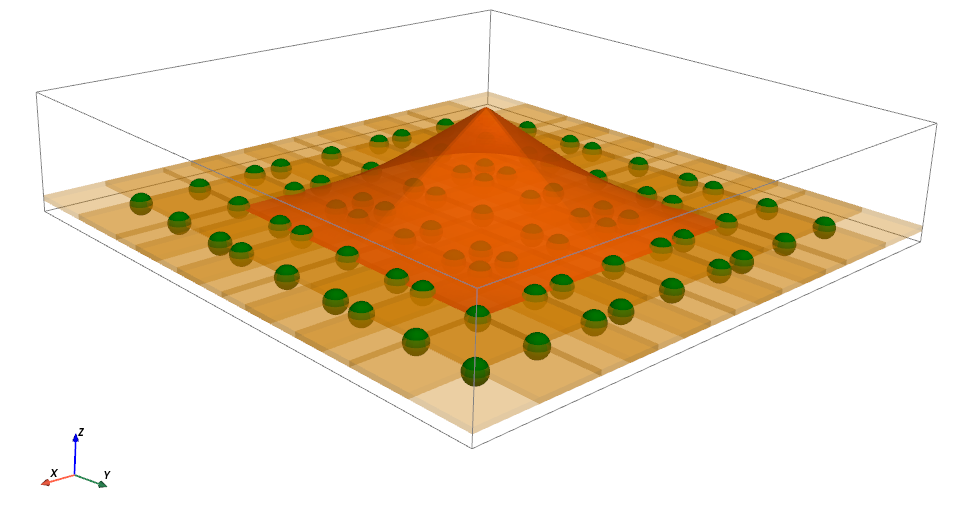
\includegraphics[width=0.6\textwidth]{Figs/mpm_basis/mpm_basis.png}
  \caption{Linear grid node shape functions for 2D traditional \MPM.}
  \label{Fig:MPMBasis2D}
\end{figure}

\subsection{MPM}
When the choice of characteristic function is the Dirac delta,
\begin{equation}\label{MPM_char}
\chi_p(\Bx) = \delta(\Bx-\Bx_p)V_p , 
\end{equation}
where $\Bx_p$ is the particle position, and $V_p$ is the particle volume,
then traditional \MPM is recovered.  In that case, the effective shape function
is still that given by Equation~\eqref{linear_shape}.  Its gradient is given by:
\begin{equation} \label{linear_shape_grad}
G_g\left(x\right) = \begin{cases} {1 / h} & {-h < x-x_g \le 0} \\
                    {-1 / h} & {0  < x-x_g \le h} \\
                    0 & \text{otherwise},
       \end{cases}
\end{equation}
Plots of Equations~\ref{linear_shape} and~\ref{linear_shape_grad} are shown
below.  The discontinuity in the gradient gives rise to poor accuracy and
stability properties.
\begin{figure}[htbp!]
  \begin{subfigure}[t]{0.5\textwidth}
    \centering
    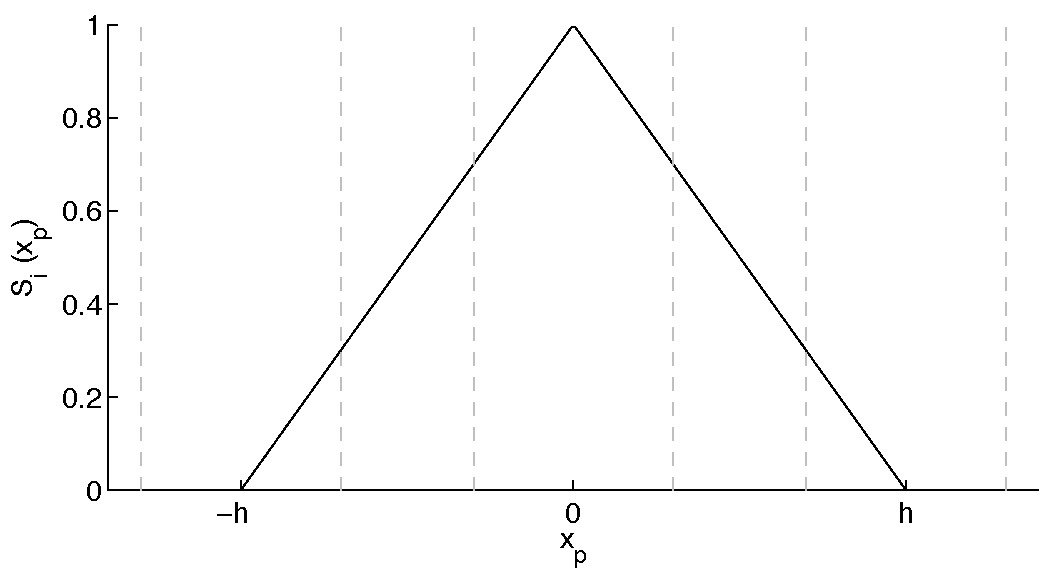
\includegraphics[width=0.9\textwidth]{mpm_basis.pdf}
    \caption{Effective shape function when using traditional \MPM.}
  \end{subfigure}
  \begin{subfigure}[t]{0.5\textwidth}
    \centering
    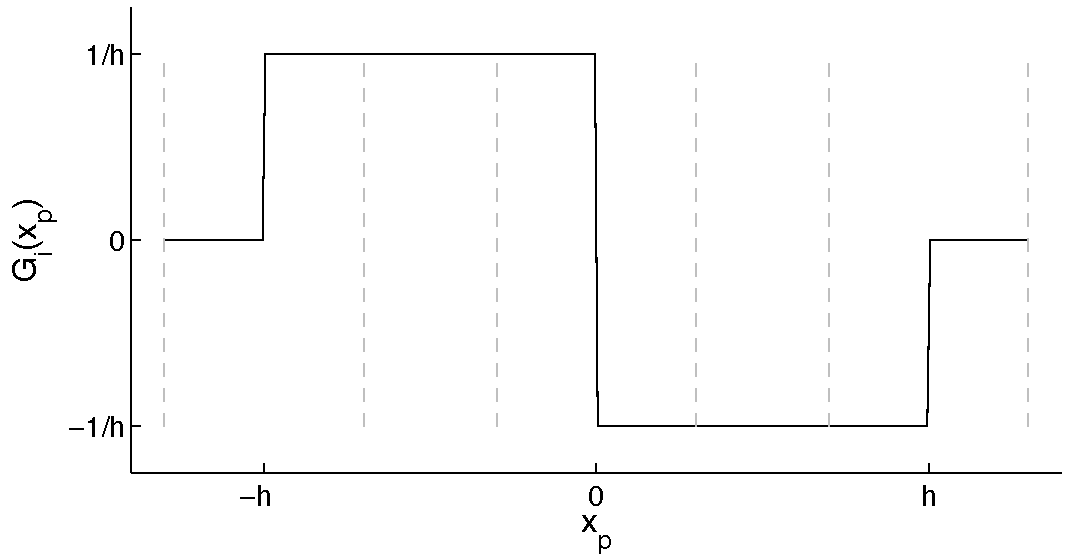
\includegraphics[width=0.9\textwidth]{mpm_grad.pdf}
    \caption{Gradient of the effective shape function when using traditional \MPM.}
  \end{subfigure}
  \label{Fig:MPMShape}
\end{figure}

\subsection{GIMP}
Typically, when an analyst indicates that
they are ``using \GIMP" this implies use of the linear grid basis function
given in Eq.~\ref{linear_shape} and a ``top-hat" characteristic function,
given by (in one-dimension),
\begin{equation} \label{GIMP_char}
\chi_p(x) = H(x-(x_p-l_p))-H(x-(x_p+l_p)) ,
\end{equation}
where $H(x)$ is the Heaviside function
($H(x)=0$ if $x<0$ and $H(x)=1$ if $x\ge0$) and $l_p$ is the half-length
of the particle.  When the convolution indicated in Eq.~\ref{effectiveS}
is carried out using the expressions in Eqns.~\ref{linear_shape}
 and~\ref{GIMP_char}, a closed form for the effective shape function can be
written as:
\begin{equation} \label{gimp_shape}
\bar{S}_{gp}\left(x_p\right) = \begin{cases}
   \frac{\left(h+l_p+\left(x_p-x_g\right)\right)^2}{4hl_p} & {-h -l_p < x_p-x_g \le -h+l_p} \\
   1 + \frac{\left(x_p-x_g\right)}{h} & {-h + l_p < x_p-x_g \le -l_p} \\
   1 - \frac{\left(x_p-x_g\right)^2 + l_p^2}{2hl_p} & {-l_p < x_p-x_g \le l_p} \\
   1 - \frac{\left(x_p-x_g\right)}{h} & {l_p  < x_p-x_g \le h-l_p} \\
   \frac{\left(h+l_p-\left(x_p-x_g\right)\right)^2}{4hl_p} & {h -l_p < x_p-x_g \le h+l_p} \\
   0 & \text{otherwise},
\end{cases}
\end{equation}
The gradient of which is:
\begin{equation} \label{gimpGrad}
\bar{G}_{gp}(x_p) = \begin{cases}
   \frac{h+l_p+\left(x_p-x_g\right)}{2 h l_p} & {-h -l_p < x_p-x_g \le -h+l_p} \\
   \frac{1}{h} & {-h + l_p < x_p-x_g \le -l_p} \\
   - \frac{\left(x_p-x_g\right)}{h l_p} & {-l_p < x_p-x_g \le l_p} \\
   - \frac{1}{h} & {l_p  < x_p-x_g \le h-l_p} \\
   - \frac{h+l_p-\left(x_p-x_g\right)}{2 h l_p} & {h -l_p < x_p-x_g \le h+l_p} \\
   0 & \text{otherwise},
\end{cases}
\end{equation}
Plots of Equations~\ref{gimp_shape} and~\ref{gimpGrad} are shown
in Figure~\ref{Fig:GIMP}.  The continuous nature of the gradients are largely responsible
for the improved robustness and accuracy of \GIMP over \MPM.
\begin{figure}[htbp!]
  \begin{subfigure}[t]{0.45\textwidth}
    \centering
    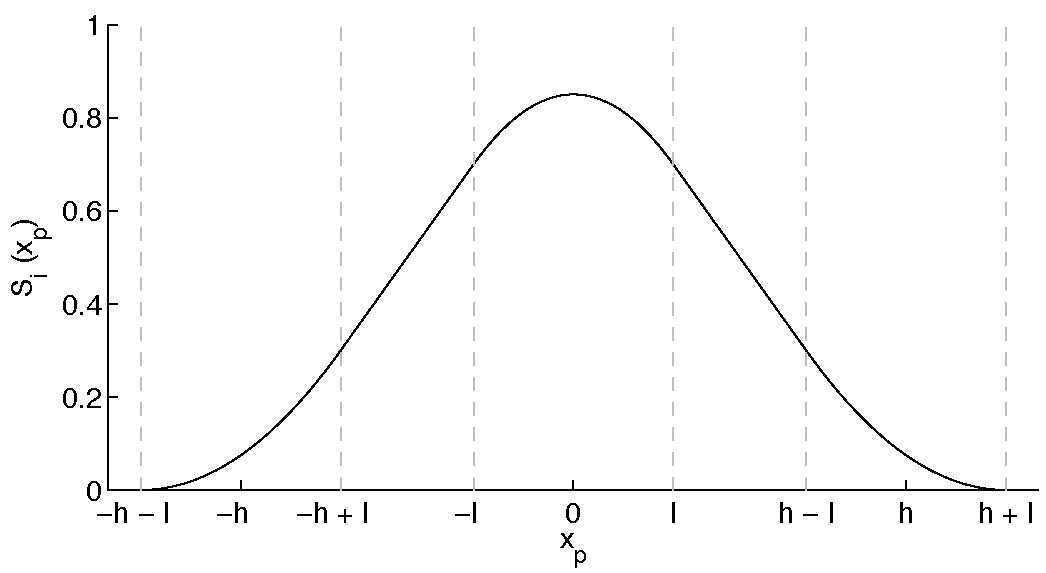
\includegraphics[width=0.9\textwidth]{gimp_basis.pdf}
    \caption{One-dimensional shape function.}
  \end{subfigure}
  \begin{subfigure}[t]{0.45\textwidth}
    \centering
    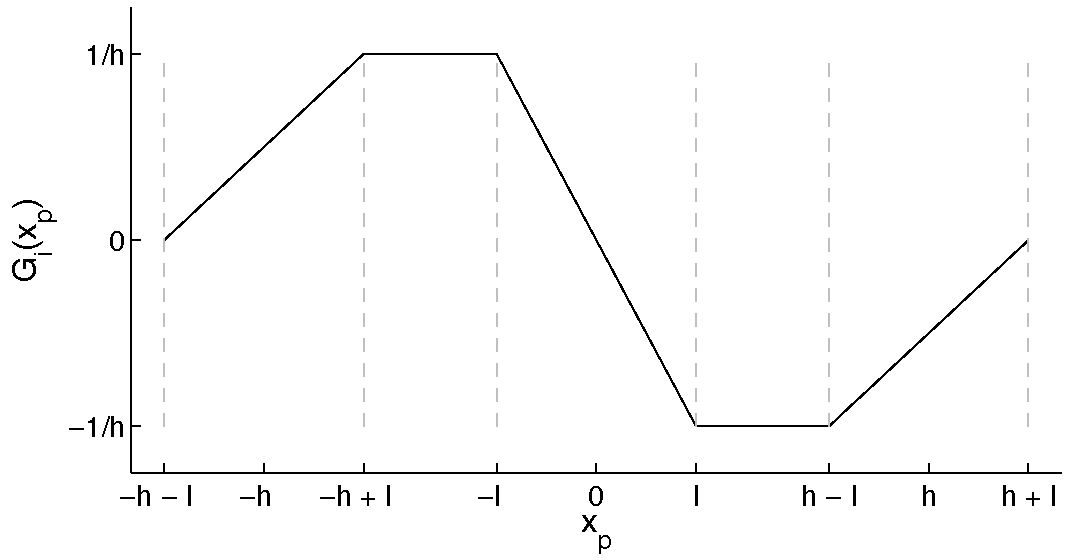
\includegraphics[width=0.9\textwidth]{gimp_grad.pdf}
    \caption{Gradient of the one-dimensional shape function.}
  \end{subfigure}
  \begin{subfigure}[t]{0.5\textwidth}
    \centering
    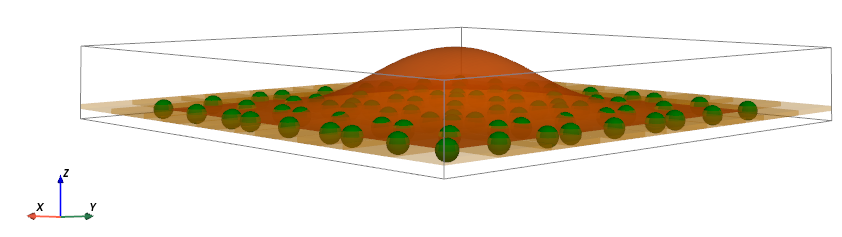
\includegraphics[width=0.9\textwidth]{Figs/mpm_basis/gimp_basis_only.png}
    \caption{Two-dimensional shape function.}
  \end{subfigure}
  \begin{subfigure}[t]{0.5\textwidth}
    \centering
    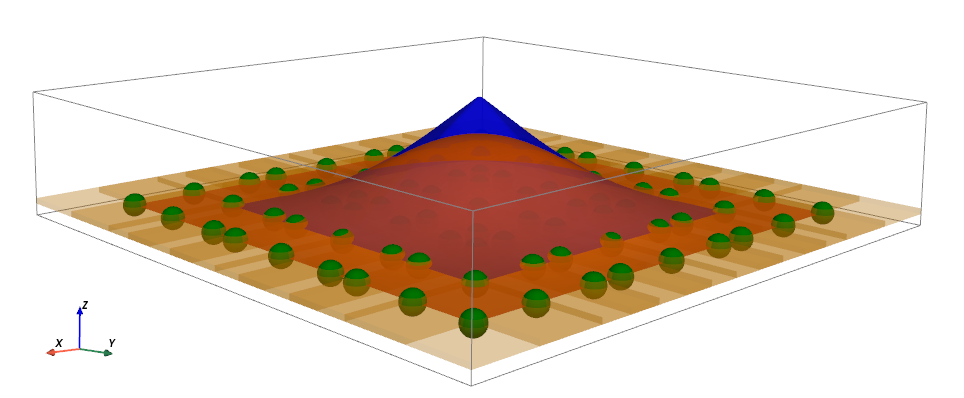
\includegraphics[width=0.9\textwidth]{Figs/mpm_basis/gimp_basis.png}
    \caption{Two-dimensional \GIMP compared to \MPM (blue).}
  \end{subfigure}
  \caption{\GIMP effective shape functions and their gradients.} 
  \label{Fig:GIMP}
\end{figure}
%
\subsection{UGIMP and cpGIMP}
The GIMP effective shape functions in \eqref{gimp_shape} are valid only for
particle sizes that are smaller than the grid spacing.  In Figure~\ref{fig:gimp_large}
we see that discontinuities appear in the effective shape function for particles for 
which $l_p > 0.5 h$.
\begin{figure}[htbp!]
  \centering
  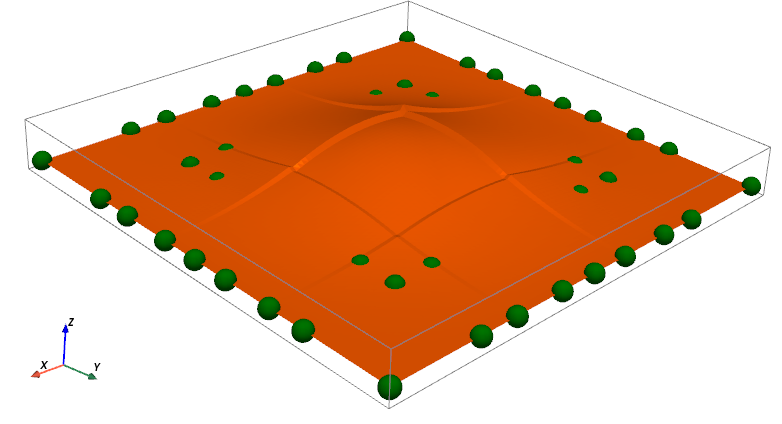
\includegraphics[width=0.6\textwidth]{Figs/mpm_basis/gimp_basis_large_particles.png}
  \caption{Two-dimensional \GIMP effective shape functions ($\bar{S}_{gp}$) for $l_p = 0.7 h$ .}
  \label{fig:gimp_large}
\end{figure}
\begin{NoteBox}
There is one further consideration in defining the effective shape function,
and that is whether or not the size (length in 1-D) of the particle is kept
fixed (denoted as \Textsfc{UGIMP} here)
or is allowed to evolve due to material deformations 
(``Finite GIMP'' or ``Contiguous GIMP'' and \Textsfc{cpGIMP} here).
In one-dimensional
simulations, evolution of the particle (half-)length is straightforward,
\begin{equation} \label{particle_length}
l_p^n = \BF_p^n l_p^0 , 
\end{equation} 
where $\BF_p^n$ is the deformation gradient at time $n$. A similar approach is used
in \Textsfc{CPDI}.
\end{NoteBox}

In multi-dimensional simulations, a similar approach can be used, assuming
an initially rectangular or cuboid particle, to find the current particle
shape.  The difficulty arises in evaluating Eq.~\eqref{effectiveS} for
these general shapes.  One approach, apparently effective, has been to create
a cuboid that circumscribes the deformed particle shape~\cite{jinmaCMES2006}.
Alternatively, one can assume that the particle size remains constant (insofar
as it applies to the effective shape function evaluations only).

\subsection{CPDI}
The \CPDI formulation~\cite{Sadeghirad2011} is a more recent method for calculating  
the quantities
\Beq \label{eq:cpdi_int}
   \Av{S_{gp}} = \frac{1}{V_p} \IntOmegap Y_p(\Bx)~\tilde{S}_g(\Bx)~d\Omega 
   \quad \Tand \quad
   \Av{\Grad{S_{gp}}} = \frac{1}{V_p} \IntOmegap Y_p(\Bx)~\Grad{\tilde{S}_g(\Bx)}~d\Omega 
\Eeq
where $Y_p$ are the particle basis functions and $\tilde{S}_g$ are approximate
grid basis functions.  Figure~\ref{fig:CPDI} shows examples of two-dimensional grid and 
particle basis functions that are used in \CPDI.
\begin{figure}[htbp!]
  \begin{subfigure}[t]{0.5\textwidth}
    \centering
    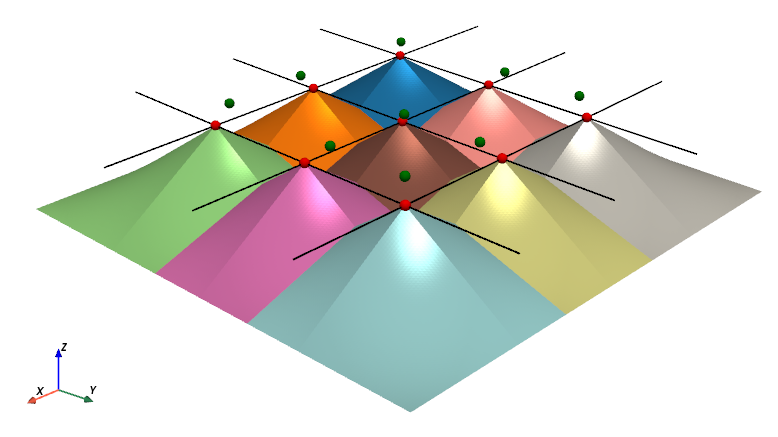
\includegraphics[width=0.9\textwidth]{Figs/mpm_basis/cpdi_grid_basis.png}
    \caption{\CPDI grid basis functions ($S_g(\Bx)$).}
  \end{subfigure}
  \begin{subfigure}[t]{0.5\textwidth}
    \centering
    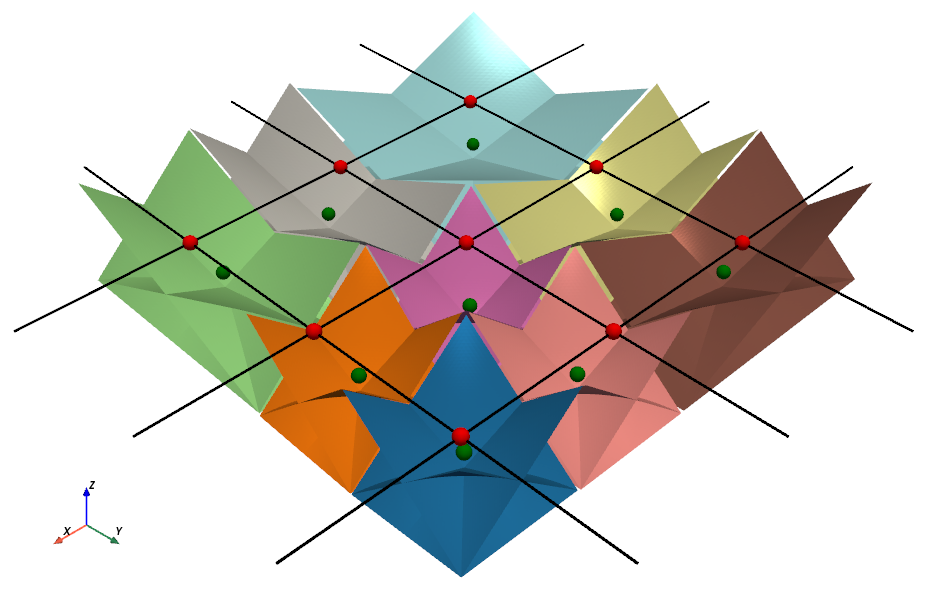
\includegraphics[width=0.9\textwidth]{Figs/mpm_basis/cpdi_particle_basis.png}
    \caption{\CPDI particle basis functions ($N_p(\Bx)$).}
  \end{subfigure}
  \caption{Two-dimensional \CPDI grid and particle basis functions.} 
  \label{fig:CPDI}
\end{figure}

In the reference state, the domain $\Omega_{p0}$ for particle $p$ is assumed to be
a parallelepiped spanned by the three vectors $\Br_p^{i0}, i=1,2,3$ with origin at the
centroid.  In the deformed
state, these vectors become $\Br_p^i = \BF_p\cdot\Br_p^{i0}$ where $\BF_p$ is the
deformation gradient.  The corners of the deformed parallelepiped are used in
CPDI to create the grid basis functions:
\Beq \label{eq:cpdi}
  \tilde{S}_g(\Bx) = \sum_{\alpha=1}^8 N_p^\alpha(\Bx) S_g(\Bx_p^\alpha)
  \quad \text{on}~\Omega_p
\Eeq
where $\alpha$ are the indices of the vertices of the particle parallelepiped,
\Beq
  N_p^\alpha(r, s, t) = \frac{1}{8}(1 + r\, r_\alpha)(1 + s\, s_\alpha)(1 + t\,t_\alpha)
\Eeq
and $r, s, t$ the natural coordinates of the parallelepiped that range from -1 to 1.
The functions $S_g(\Bx)$ are typically chosen to be the hat functions of classical
MPM.  Figure~\ref{fig:cpdi_eff} shows the particle domains and the effective grid
shape functions produced by the \CPDI relation in \eqref{eq:cpdi}.
\begin{figure}[htbp!]
  \begin{subfigure}[t]{0.5\textwidth}
    \centering
    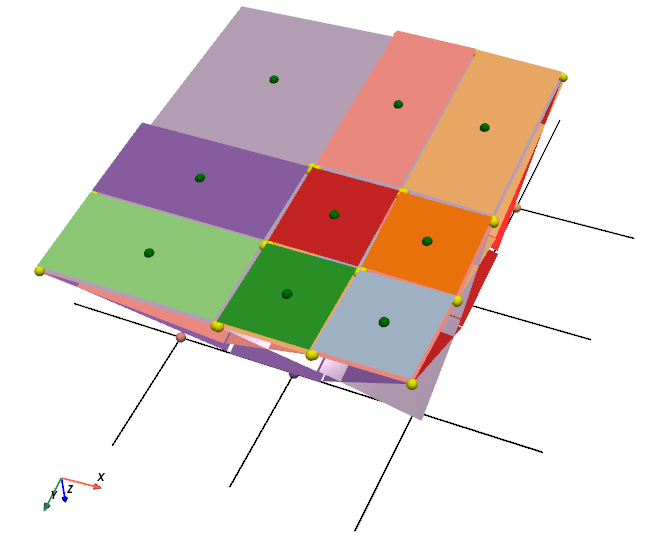
\includegraphics[width=0.9\textwidth]{Figs/mpm_basis/cpdi_particle_domains.png}
    \caption{Particle domains $\Omega_p$.}
  \end{subfigure}
  \begin{subfigure}[t]{0.5\textwidth}
    \centering
    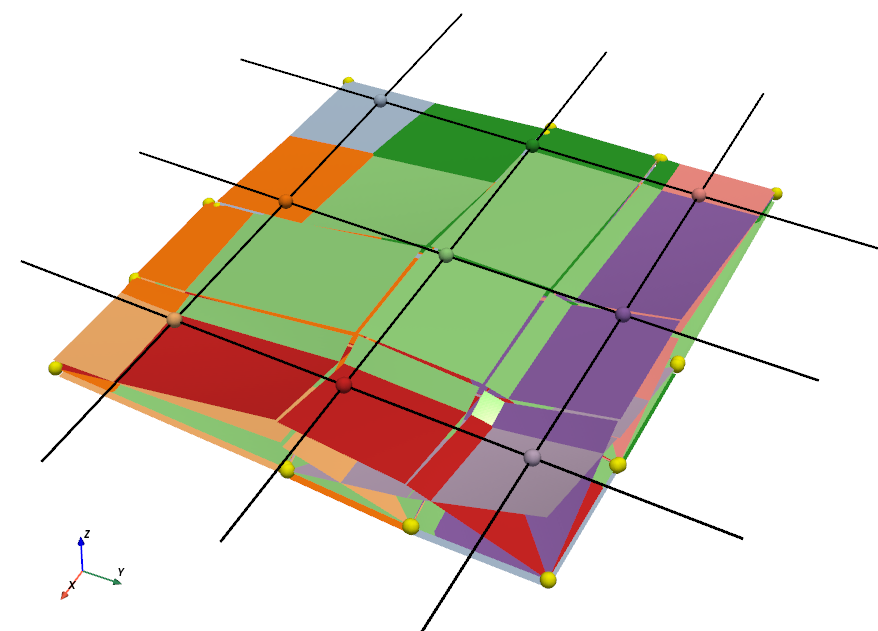
\includegraphics[width=0.9\textwidth]{Figs/mpm_basis/cpdi_effective_basis.png}
    \caption{Effective grid basis functions ($\tilde{S}_g(\Bx)$).}
  \end{subfigure}
  \caption{Two-dimensional \CPDI particle domains and effective grid basis functions.} 
  \label{fig:cpdi_eff}
\end{figure}


We can compute the quantities in \eqref{eq:cpdi_int} as follows.

Let
\Beq
  \Bsv_p^0 = \begin{bmatrix} \Br_p^{10} & \Br_p^{20} & \Br_p^{30} \end{bmatrix} \quad \Tand \quad
  \Bsv_p = \begin{bmatrix} \Br_p^1 & \Br_p^2 & \Br_p^3 \end{bmatrix} \quad \Tand \quad
  \BFv_p = \begin{bmatrix} F_{11} & F_{12} & F_{13} \\
                           F_{21} & F_{22} & F_{23} \\ F_{31} & F_{32} & F_{33} 
                           \end{bmatrix} \,.
\Eeq
Then $ \Bsv_p = \BFv_p \Bsv_p^0$.  Let
\Beq
  \BSv_{gp} = \begin{bmatrix}
               S_g(\Bx_p^1) & S_g(\Bx_p^2) & S_g(\Bx_p^3) & S_g(\Bx_p^4) & 
               S_g(\Bx_p^5) & S_g(\Bx_p^6) & S_g(\Bx_p^7) & S_g(\Bx_p^8) 
             \end{bmatrix} \,.
\Eeq
Also, let
\Beq
  \BRv = \begin{bmatrix}
           -1 &  1 &  1 & -1 & -1 &  1 &  1 & -1 \\ 
           -1 & -1 &  1 &  1 & -1 & -1 &  1 &  1 \\ 
           -1 & -1 & -1 & -1 &  1 &  1 &  1 &  1
         \end{bmatrix}
\Eeq
Then,
\Beq
  \overbar{S}_{gp} = \Av{S_{gp}} = \text{mean}(\BSv_{gp})
  \quad \Tand \quad
  \overbar{\BG}_{gp} = \Av{\Grad{S_{gp}}} = \frac{1}{8} \Bsv_p^{-T} \BRv^T \BSv_{gp}^T \,.
\Eeq

\section{Contact algorithms}
The default behavior of \MPM is to handle interactions between objects using velocities on
the background grid.  However, beyond some simple situations, contact requires the application
of contact laws.  In the \Vaango implementation of friction contact, Coulomb friction is
assumed.  Alternative types of contact, such as adhesive contact. could also be implemented by
changing the contact law.

The purpose of the various contact algorithms in \Vaango is to correct the grid velocities
such that a particular set of contact assumptions are satisfied.  The two main algorithms
are \Textsfc{friction\_bard}, which is based on~\cite{Bard2001}, and \Textsfc{friction\_LR},
which is described in~\cite{Nairn2020}.

Let $m_p$, $\Bv_p$, $\Bp_p$ be the mass, velocity, and momentum of particle $p$. Also, let $m_g$,
$\Bv_g$, $\Bp_g$ be the mass, velocity, and momentum at a grid point $g$ due to nearby particles
in the region of influence.  Consider $N_\alpha$ objects that can potentially be in contact and index
then by the superscript $\alpha$.
Then, from \eqref{eq:vol_weighted_mom}, we have
\Beq
  m_g^\alpha = V_g^\alpha \rho_g^\alpha = \sum_p V_p^\alpha \rho_p^\alpha \bar{S}_{gp}
             = \sum_p m_p^\alpha \bar{S}_{gp} \quad \Tand \quad
  \Bp_g^\alpha = \sum_p \Bp_p^\alpha \bar{S}_{gp} \,.
\Eeq
In matrix notation,
\Beq
  \BmT_g^\alpha = \SfS^T \BmT_p^\alpha \quad \Tand \quad
  \BpT_g^\alpha = \SfS^T \BpT_p^\alpha \,.
\Eeq
Similarly, from \eqref{eq:mass_weighted_vel}, we have
\Beq 
  m_g^\alpha \Bv_g^\alpha = \sum_p m_p^\alpha \Bv_p^\alpha \bar{S}_{gp}
  \quad \implies \quad
  \Bv_g^\alpha = \frac{1}{m_g^\alpha} \sum_p m_p^\alpha \Bv_p^\alpha \bar{S}_{gp} \,.
\Eeq
In matrix form,
\Beq
  \BvT_g^\alpha = \SfS^\plus_\alpha \BvT_p^\alpha 
  \quad \text{where} \quad
  \SfS^\plus_\alpha = \left(\BmT_g^\alpha\right)^{-1} \SfS^T \BmT_p^\alpha \,.
\Eeq
Based on a local conservation of momentum, we define a {\em center-of-mass} velocity, $\Bv_g^{\Tcm}$,
at grid node $g$ for all the contacting objects:
\Beq \label{eq:center_of_mass_vel}
  \Bv_g^{\Tcm} = \frac{\sum_\alpha m_g^\alpha \Bv_g^\alpha}{\sum_\alpha m_g^\alpha} \,.
\Eeq
We also define an effective grid mass, $m_g^\Teff$, as
\Beq \label{eq:eff_mass}
  \frac{1}{m_g^\Teff} = \sum_\alpha \frac{1}{m_g^\alpha} \,.
\Eeq

\subsection{Bardenhagen et al. algorithm}
In the algorithm developed in~\cite{Bard2001}, a contact interface is defined as the set of
nodes for which individual grid velocities associated with each object differ from the
center of mass velocity:
\Beq
  \Bv_g^\alpha - \Bv_g^\Tcm \ne 0 \,.
\Eeq
Once this condition is identified, the surface normal $\Bn_g^\alpha$ is computed
from the mass distribution around node $g$, and the surface normal traction
$\Bt_g^\alpha$ is computed from the stresses in surrounding material points.

The contact condition is
\Beq \label{eq:contact_constraint_bard}
(\Bv_g^\alpha - \Bv_g^\Tcm)\cdot\Bn_g^\alpha > 0 \quad \Tand \quad
\Bt_g^\alpha \cdot \Bn_g^\alpha < 0 \,.
\Eeq
This condition indicates compressive stress at node $g$.  If this condition is not satisfied,
the objects are assumed to have separated.

To enforce \eqref{eq:contact_constraint_bard}, the grid node velocities are adjusted
such that momentum is conserved, i.e.,
\Beq
  \Delta (v_n)_g^\alpha = \Delta \Bv_g^\alpha \cdot \Bn_g^\alpha \quad \Tand \quad
  \Delta (v_t)_g^\alpha = \Delta \Bv_g^\alpha \cdot \left[
     \Bn_g^\alpha \times \frac{\Delta \Bv_g^\alpha \times \Bn_g^\alpha}%
                              {\Norm{\Delta \Bv_g^\alpha \times \Bn_g^\alpha}{}} \right]
\Eeq
where
\Beq
  \Delta \Bv_g^\alpha := \Bv_g^\alpha - \Bv_g^\Tcm \,.
\Eeq
Normal contact is enforced by adjusting material velocities by $\Delta (v_n)_g^\alpha$.
The tangential contact is enforced using Coulomb friction with the tangential velocity
determined using $\mu \Delta (v_n)_g^\alpha$ where $\mu$ is the friction coefficient. If
$\Delta (v_t)_g^\alpha < \mu \Delta (v_n)_g^\alpha$, the no-slip condition is enforced.
Otherwise, the tangential components of the nodal velocities are updated with a reduced
friction coefficient
\Beq
  \mu_\Tred = \Tmin\left(\mu, \frac{|\Delta (v_t)_g^\alpha|}{|\Delta (v_n)_g^\alpha|}\right) \,.
\Eeq

Returning to the problem of computing object outward normals at a grid point, the
traditional approach is to compute volume gradients using the set of particles influencing
a node:
\Beq
  \Bg_g^\alpha = \sum_{p^\alpha} \overbar{\BGv}_{gp} V_p 
\Eeq
where the gradients $\overbar{\BGv}_{gp}$ are as defined in \eqref{eq:G_mpm}, \eqref{eq:G_gimp}, and
\eqref{eq:G_cpdi}.  The normal to an object is calculated using
\Beq
  \Bn^\alpha = \frac{\Bg_g^\alpha}{\Norm{\Bg_g^\alpha}{}} \,.
\Eeq
For multiple objects, an average gradient can be computed for better accuracy.

\subsection{Nairn et al. algorithm}
The more recent algorithm by~\cite{Nairn2020} uses a logistic regression step to determine
contact.  The underlying approach is similar to that used in ~\cite{Bard2001}.  Since the approach
is at its simplest when only two objects are involved at a grid point, we will describe only that
case below.  Most situations with contact between multiple objects see~\cite{Nairn2020}.

Let the two objects be indexed by $\alpha$ and $\beta$.  Let $\Bp_g^{\alpha 0}$ and $\Bp_g^{\beta 0}$
be the particle momenta projected to the grid.  We would like to compute the momentum correction
$\Delta \Bp$ so that momentum is conserved after contact.  Let the corrected momenta be
\Beq \label{eq:p_alpha_beta}
  \Bp_g^\alpha = \Bp_g^{\alpha 0} + \Delta \Bp \quad  \Tand \quad
  \Bp_g^\beta = \Bp_g^{\beta 0} - \Delta \Bp  \,.
\Eeq
If we restrict relative motion between objects at a grid point to the tangent plane, and let
$\Bthat$ be the direction of relative motion, then
\Beq \label{eq:v_alpha_beta}
  \Bv_g^\beta - \Bv_g^\alpha = k \Bthat \quad \implies \quad
  \frac{\Bp_g^\beta}{m_g^\beta} - \frac{\Bp_g^\alpha}{m_g^\alpha} = k \Bthat
  \quad \implies \quad
  m_g^\alpha \Bp_g^\beta - m_g^\beta \Bp_g^\alpha = m_g^\alpha m_g^\beta k \Bthat \,.
\Eeq
From the definition of the center-of-mass velocity in \eqref{eq:center_of_mass_vel} and
the effective grid mass~\eqref{eq:eff_mass}, we have
\Beq 
  \Bv_g^{\Tcm} = \frac{m_g^\alpha \Bv_g^\alpha + m_g^\beta \Bv_g^\beta}{m_g^\alpha + m_g^\beta} 
     = \frac{\Bp_g^\alpha + \Bp_g^\beta}{m_g^\alpha + m_g^\beta}  \quad \Tand \quad
  m_g^\Teff = \frac{m_g^\alpha m_g^\beta}{m_g^\alpha + m_g^\beta} \,.
\Eeq
Therefore,
\Beq \label{eq:p_alpha_beta_1}
  \Bp_g^\alpha + \Bp_g^\beta =  \frac{\Bv_g^{\Tcm} m_g^\alpha m_g^\beta}{m_g^\Teff} \,.
\Eeq
Solving for $\Bp_g^\alpha, \Bp_g^\beta$ from equations \eqref{eq:v_alpha_beta} and
\eqref{eq:p_alpha_beta_1}, we have
\Beq
  \Bp_g^\alpha = m_g^\alpha \Bv_g^\Tcm - m_g^\Teff k \Bthat \quad \Tand \quad
  \Bp_g^\beta = m_g^\beta \Bv_g^\Tcm + m_g^\Teff k \Bthat \,.
\Eeq
Therefore, from \eqref{eq:p_alpha_beta},
\Beq
\Delta \Bp = \Bp_g^\alpha - \Bp_g^{\alpha 0}
           = m_g^\alpha \Bv_g^\Tcm - m_g^\Teff k \Bthat - m_g^\alpha \Bv_g^{\alpha 0} 
           = m_g^\alpha (\Bv_g^\Tcm - \Bv_g^{\alpha 0}) - m_g^\Teff k \Bthat \,.
\Eeq
The quantity
\Beq
  \Delta \Bp^0 := m_g^\alpha (\Bv_g^\Tcm - \Bv_g^{\alpha 0})
\Eeq
is the initial change of momentum before tangential correction.
Since the contact force ($\Bf^c$) is given by the rate of change of momentum due to contact, we
have
\Beq
  \Bf^{c0} = \frac{\Delta \Bp^0}{\Delta t} \quad \Tand \quad
  \Bf^c = \frac{\Delta \Bp}{\Delta t} = \Bf^{c0} - \frac{m_g^\Teff k \Bthat}{\Delta t} \,.
\Eeq
where $\Delta t$ is the timestep size.
The contact compressive traction is found from the normal component of the contact force needed to
prevent interpenetration:
\Beq
  T^c_n = -\frac{1}{A^c}\,\Bf^{c0}\cdot\Bn
\Eeq
where $A^c$ is the contact area.  The tangential contact traction can be found using a
contact law:
\Beq
  T^c_t = \frac{1}{A^c}\,\Bf^c\cdot\Bthat
        = \frac{1}{A^c}\left[\Bf^{c0}\cdot\Bthat - \frac{m_g^\Teff k}{\Delta t}\right] \,.
\Eeq
Therefore, if $T^c_t = T^c_t(T^c_n)$ is a contact law, 
\Beq
  k = \frac{\Delta t}{m_g^\Teff} \left[\Bf^{c0} \cdot \Bthat - A^c T^c_t(T^c_n)\right] \,.
\Eeq
We can compute $k$ using the contact law $T^c_t(T^c_n)$ and then adjust $\Bv_g^\alpha$
and $\Bv_g^\beta$ using \eqref{eq:p_alpha_beta}.  Note that this process is identical to that
used in the Bardenhagen at al. algorithm.  The main difficulty is in finding where contact has occurred
and the quantities $\Bn$, $\Bthat$, and $A^c$.




\section{Implicit time integration}
Recall from equation~\eqref{eq:discrete_MPM_equations} that the \MPM discretized momentum
equations can be written as a semi-algebraic system
\Beq \label{eq:discrete_MPM_equations_1}
  \sum_h M_{gh} \dot{\Bv}_h = \Bf_g^{\Text} -\Bf_g^{\Tint} + \Bf_g^{\Tbody} 
      ~;~~ g = 1 \dots N_g
\Eeq
where the mass matrix ($\BM$), the internal force vector ($\Bf_g^{\Tint}$), 
the body force vector ($\Bf_g^{\Tbody}$), and the  external force vector ($\Bf_g^{\Text}$)
at grid node $g$ as
\Beq \label{eq:fext_fint_def}
  \Bal
   &M_{gh} := \sum_p \rho_p\IntOmegap Y_p(\Bx)~S_g(\Bx)~S_h(\Bx)~d\Omega \\
   &\Bf_g^{\Tint} := \sum_p V_p \Bsig_p \cdot \Av{\Grad{S_{gp}}} \\
   &\Bf_g^{\Tbody} := \sum_p m_p\Bb_p~\Av{S_{gp}} \\
   &\Bf_g^{\Text} := \IntGammat \Bart(\Bx)~S_g(\Bx)~d\Gamma \,.
  \Eal
\Eeq

While the \MPM background grid is reset after each time increment, \MPM does not
require it to be reset during each iteration of an implicit integration process.
Therefore, during a time step, we can carry a grid displacement variable $\Bu$ that 
can be used to compute grid accelerations $\Ba_g = \dot{\Bv}_g$ and discarded at
the end of a time step.

Let us express \eqref{eq:discrete_MPM_equations_1} in matrix form as
\Beq
  \BM_g \BaT_g = \BfT_g^{\Text} - \BfT_g^{\Tint} + \BfT_g^{\Tbody} 
\Eeq
Define the residual as
\Beq \label{eq:mpm_residual}
  \Br(\BuT_g^{n+1}, t_{n+1}) = \BM_g \BaT_g^{n+1} - \BfT^{\Text}(\BuT_g^{n+1}, t_{n+1}) + 
     \BfT^{\Tint}(\BuT_g^{n+1}, t_{n+1}) - \BfT^{\Tbody}(\BuT_g^{n+1}, t_{n+1}) = \Bzero .
\Eeq
where the superscipt $n+1$ indicates quantities at time $t_{n+1}$ and $\BuT_g$ is the 
$N_g \times 3$ matrix of grid
node displacements.  We use a Newmark-$\beta$ method to integrate the acceleration:
\Beq \label{eq:newmark_beta}
  \Bal
    \BuT_g^{n+1} & = \BuT^\star + \beta  \BaT_g^{n+1} (\Delta t)^2 \\
    \BvT_g^{n+1} & = \BvT^\star + \gamma \BaT_g^{n+1} \Delta t 
  \Eal
\Eeq
where
\Beq
  \Bal
    \BuT^\star & = \BuT_g^n + \BvT_g^n \Delta t + \Half (1 - 2\beta) \BaT_g^n (\Delta t)^2 \\
    \BvT^\star & = \BvT_g^n + (1 - \gamma) \BaT_g^n \Delta t \,.
  \Eal
\Eeq

\subsection{Newton's method}
In the \Vaango implementation, the residual is expressed in terms of the displacement.  
We are required to do this because tangents needed in Newton's method are easier to compute 
when forces can be expressed in the form
\Beq
  \BfT = \BK \cdot \BuT
\Eeq
where $\BK$ is the stiffness matrix.  If we were to use the velocity as the primary variable,
as in explicit MPM, we would need rates of the forces instead:
\Beq
  \dot{\BfT} = \BK \cdot \BvT + \dot{\BK} \cdot \BuT \,.
\Eeq
The extra term involving the rate of change of the stiffness matrix complicates the process
and we avoid it in \Vaango.

Then, using \eqref{eq:mpm_residual} and \eqref{eq:newmark_beta}, we have
\Beq \label{eq:mpm_residual_1}
  \Br(\BuT_g^{n+1}, t_{n+1}) = \frac{1}{\beta \Delta t^2} \BM_g (\BuT_g^{n+1} - \BuT^\star) - 
      \BfT^{\Text}(\BuT_g^{n+1}, t_{n+1}) + 
     \BfT^{\Tint}(\BuT_g^{n+1}, t_{n+1}) - \BfT^{\Tbody}(\BuT_g^{n+1}, t_{n+1}) = \Bzero .
\Eeq
The problem then reduces to finding the solution $\BuT_g^{n+1}$ of the nonlinear system of equations
\eqref{eq:mpm_residual_1}. Newton's method is used in \Vaango with the starting 
value of $\BuT_g^{n+1} = \BuT_g^\star$.  Dropping the subscript $g$ temporarily for convenience,
and denoting the current Newton iteration by the subscript $k$, we can linearize the residual at 
$\BuT_k^{n+1}$ using a Taylor expansion:
\Beq
  \Bzero = \Br(\BuT_{k+1}^{n+1}, t_{n+1}) = 
     \Br(\BuT_k^{n+1}, t_{n+1}) + \Partial{\Br(\BuT_k^{n+1}, t_{n+1})}{\BuT}(\BuT^{n+1}_{k+1} - \BuT^{n+1}_k) \,.
\Eeq
Rearranging the above equation,
\Beq \label{eq:Newton_step}
  \Delta\BuT = \BuT^{n+1}_{k+1} - \BuT^{n+1}_k = 
     -\left[\Partial{\Br(\BuT_k^{n+1}, t_{n+1})}{\BuT}\right]^{-1}
     \Br(\BuT_k^{n+1}, t_{n+1})  = -\BK^{-1} \Br(\BuT_k^{n+1}, t_{n+1})\,.
\Eeq
This iterative process is continued until $\Delta \BuT$ is smaller than a given tolerance.
The tangent matrix $\BK$, of size $N_g \times N_g$, is 
\Beq
  \BK = \Partial{\Br(\BuT_k^{n+1}, t_{n+1})}{\BuT} \,.
\Eeq
This matrix is decomposed and evaluated separately for the internal and external forces, i.e., 
\Beq
  \BK = \Partial{\Br(\BuT_k^{n+1}, t_{n+1})}{\BuT} 
      = \frac{1}{\beta \Delta t^2} \BM_g  - \Partial{}{\BuT}\left[\BfT^{\Text}(\BuT_g^{n+1}, t_{n+1})\right] + 
        \Partial{}{\BuT}\left[\BfT^{\Tint}(\BuT_g^{n+1}, t_{n+1})\right] - 
        \Partial{}{\BuT}\left[\BfT^{\Tbody}(\BuT_g^{n+1}, t_{n+1})\right] \,.
\Eeq
Alternatively,
\Beq
  \BK = \frac{1}{\beta \Delta t^2} \BM_g  - \BK^{\Text}(\BuT_g^{n+1}, t_{n+1}) +  
         \BK^{\Tint}(\BuT_g^{n+1}, t_{n+1}) -  \BK^{\Tbody}(\BuT_g^{n+1}, t_{n+1}) \,.
\Eeq

\subsection{Tangent stiffness matrix}
The contribution to the tangent matrix ($\BK$) from the internal forces is called the
\Textsfc{tangent stiffness matrix} ($\BK^\Tint$).  Since an updated Lagrangian formulation is used
in \MPM, we can compute the tangent stiffness using the configuration at time $t_n$ as
the reference configuration.

Recall from \eqref{eq:fext_fint_def} that for explicit \MPM we used
\Beq \label{eq:f_g_int_0}
  \Bf_g^{\Tint} = \sum_p V_p \Bsig_p \cdot \Av{\Grad{S_{gp}}}  
  \quad \text{where} \quad
  \Av{S_{gp}} := \frac{1}{V_p} \IntOmegap Y_p(\Bx)~S_g(\Bx)~d\Omega \,.
\Eeq
For the computation of the tangent matrix, it is preferable to start from the
weak form of the momentum equation \eqref{eq:weak_form}:
\Beq \label{eq:f_int_weak}
  I = \IntOmega \Bsig:\Grad{\Bw}~d\Omega  
\Eeq
which leads to integral form of equation \eqref{eq:f_g_int_0} (see \eqref{eq:integral_weak_form}):
\Beq  \label{eq:f_g_int}
  \Bf_g^{\Tint} = \sum_p\IntOmegap Y_p(\Bx)\Bsig_p \cdot \Grad{S_g}~d\Omega \,.
\Eeq
Also, since we are typically working with rates of stress in the constitutive models, it
is preferable to express all quantities in terms of stress rates that are objective.
It is easier to work with the Lagrangian PK-1 stress ($\BP$) at the beginning of the timestep
rather than the spatial Cauchy stress ($\Bsig$).

To convert from the spatial description \eqref{eq:f_int_weak} to a Lagrangian material 
description, observe that
\Beq
  \underset{n+1}{\nabla}{\Bw} = \Partial{\Bw}{\Bx^{n+1}} = \Partial{\Bw}{\Bx^n} \cdot \Partial{\Bx^n}{\Bx^{n+1}} 
    = \Partial{\Bw}{\Bx^n} \cdot (\Delta\BF_n^{n+1})^{-1}
    = \Partial{\Bw}{\Bx^n} \cdot \frac{\Delta\BF_c^T}{J_n^{n+1}}
    = \underset{n}{\nabla} \Bw \cdot \frac{\Delta\BF_c^T}{J_n^{n+1}}
\Eeq
where, with $\BF$ as the deformation gradient, 
\Beq
  \BF^{n+1} = \Delta\BF_n^{n+1} \BF^n~,~~ J_n^{n+1} = \det(\Delta\BF_n^{n+1}) ~,~~
  \Delta\BF_c = \text{cofactor}(\Delta\BF_n^{n+1}) \,.
\Eeq
Therefore,
\Beq
  \Bal 
   I & = \int_{\Omega^{n+1}} \Bsig^{n+1} : \underset{n+1}{\nabla}{\Bw}~d\Omega^{n+1}
       = \int_{\Omega^n} \Bsig^{n+1} : \underset{n+1}{\nabla}{\Bw}~J_n^{n+1}\,d\Omega^n \\
     & = \int_{\Omega^n} \Bsig^{n+1} : \left(\underset{n}{\nabla}{\Bw}\cdot \Delta\BF_c^T\right)\,d\Omega^n 
       = \int_{\Omega^n} \left(\Bsig^{n+1} \cdot \Delta\BF_c\right) : \underset{n}{\nabla}{\Bw}\,d\Omega^n \\
     & = \int_{\Omega^n} \BP^n : \underset{n}{\nabla}{\Bw}\,d\Omega^n 
  \Eal
\Eeq
where $\BP^n$ is the first Piola-Kirchhoff stress.  Following the same process as used to derive
\eqref{eq:integral_weak_form}, we get
\Beq  \label{eq:f_g_int_lagrangian}
  \Bf_g^{\Tint} = \sum_p\int_{\Omega_p^n} Y_p(\Bx^n)\BP_p^n \cdot \underset{n}{\nabla}{S_g}~d\Omega^n \,.
\Eeq
Taking the material time derivative of \eqref{eq:f_g_int_lagrangian}, we have
\Beq  \label{eq:rate_f_g_int_lagrangian}
  \dot{\Bf}_g^{\Tint} = \sum_p\int_{\Omega_p^n} Y_p(\Bx^n)\dot{\BP}_p^n \cdot \underset{n}{\nabla}{S_g}~d\Omega^n \,.
\Eeq
Since the rate of the first Piola-Kirchhoff stress is not objective, it is easier to work with
the rate of the second Piola-Kirchhoff stress ($\BS$):
\Beq \label{eq:rate_P}
  \BP = \BF \cdot \BS \quad \implies \quad
  \dot{\BP} = \dot{\BF} \cdot \BS + \BF \cdot \dot{\BS} \,.
\Eeq
Substitution of \eqref{eq:rate_P} into \eqref{eq:rate_f_g_int_lagrangian} gives
\Beq
  \dot{\Bf}_g^{\Tint} = \sum_p\int_{\Omega_p^n} Y_p(\Bx^n)\left[\dot{\BF}_p^{n+1} \cdot \BS_p^n + \BF_p^{n+1} \cdot \dot{\BS}_p^n\right] \cdot \underset{n}{\nabla}{S_g}~d\Omega^n \,.
\Eeq
Separating out the two components, we have
\Beq
  \dot{\Bf}_g^{\Tint} = 
    \sum_p\int_{\Omega_p^n} Y_p(\Bx^n) \dot{\BF}_p^{n+1} \cdot \BS_p^n \cdot \underset{n}{\nabla}{S_g}~d\Omega^n + 
    \sum_p\int_{\Omega_p^n} Y_p(\Bx^n) \BF_p^{n+1} \cdot \dot{\BS}_p^n \cdot \underset{n}{\nabla}{S_g}~d\Omega^n \,.
\Eeq
The rate of the internal force can then be expressed as
\Beq
  \dot{\Bf}_g^{\Tint} = \dot{\Bf}_g^{\Tgeo} + \dot{\Bf}_g^{\Tmat}
\Eeq
where the geometric and material rates of the internal forces are defined as
\Beq \label{eq:fdot_mat_geo}
  \Bal
   \dot{\Bf}_g^{\Tgeo} & :=  \sum_p\int_{\Omega_p^n} Y_p(\Bx^n) \dot{\BF}_p^{n+1} \cdot \BS_p^n \cdot \underset{n}{\nabla}{S_g}~d\Omega^n  \\
   \dot{\Bf}_g^{\Tmat} & :=  \sum_p\int_{\Omega_p^n} Y_p(\Bx^n) \BF_p^{n+1} \cdot \dot{\BS}_p^n \cdot \underset{n}{\nabla}{S_g}~d\Omega^n \,.
  \Eal
\Eeq
We can now use the constitutive relation between the second Piola-Kirchhoff stress and the
Green strain ($\BE$), the expression for the Green strain in terms of the deformation gradient,
the relationship between the velocity gradient ($\BlT$) and the rate of
change of the deformation gradient, and the definition of the rate-of-deformation ($\BdT$)
\Beq
  \dot{\BS} = \CalC : \dot{\BE}~,~~ \BE = \Half\left(\BF^T \cdot \BF - \BI\right) ~,~~
  \dot{\BF} = \BlT \cdot \BF, \quad \Tand \quad \BdT = \Half(\BlT + \BlT^T)
\Eeq
to write the material and geometric rates of the internal force in \eqref{eq:fdot_mat_geo} as
\Beq \label{eq:fdot_mat_geo_1}
  \Bal
   \dot{\Bf}_g^{\Tmat} 
   & =  \sum_p\int_{\Omega_p^n} Y_p(\Bx^n) \BF_p^{n+1} \cdot \left[\CalC_p^n : \dot{\BE}_p^n\right] 
        \cdot \underset{n}{\nabla}{S_g}~d\Omega^n  \\
   & = \Half \sum_p\int_{\Omega_p^n} Y_p(\Bx^n) \BF_p^{n+1} \cdot \left[
        \CalC_p^n :
        \left((\dot{\BF}_p^{n+1})^T \cdot \BF_p^{n+1} + (\BF_p^{n+1})^T \cdot \dot{\BF}_p^{n+1}\right)
        \right] \cdot \underset{n}{\nabla}{S_g}~d\Omega^n  \\
   & = \Half \sum_p\int_{\Omega_p^n} Y_p(\Bx^n) \BF_p^{n+1} \cdot \left[
        \CalC_p^n :
        \left((\BF_p^{n+1})^T \cdot (\BlT_p^{n+1})^T \cdot \BF_p^{n+1} +
              (\BF_p^{n+1})^T \cdot \BlT_p^{n+1} \cdot \BF_p^{n+1}\right)
        \right] \cdot \underset{n}{\nabla}{S_g}~d\Omega^n  \\
   & = \sum_p\int_{\Omega_p^n} Y_p(\Bx^n) \BF_p^{n+1} \cdot \left[
        \CalC_p^n :
        \left((\BF_p^{n+1})^T \cdot \BdT_p^{n+1} \cdot \BF_p^{n+1}\right)
        \right] \cdot \underset{n}{\nabla}{S_g}~d\Omega^n  \\
   \dot{\Bf}_g^{\Tgeo} & :=
     \sum_p\int_{\Omega_p^n} Y_p(\Bx^n) \left[(\BF_p^{n+1})^T \cdot (\BlT_p^{n+1})^T\right] \cdot \BS_p^n \cdot \underset{n}{\nabla}{S_g}~d\Omega^n \,.
  \Eal
\Eeq
Recall the interpolation of the velocity from the grid nodes ($h$) to particles ($p$) can be
computed using
\Beq
  \Bv_p(\Bx^{n+1}) = \sum_h \Bv_h^{n+1} S_h(\Bx^{n+1})
\Eeq
Therefore,
\Beq \label{eq:vel_grad_implicit}
  \Bal
  \BlT_p^{n+1} & = \underset{n+1}{\nabla}\Bv_p^{n+1}(\Bx^{n+1}) = 
    \sum_h \Bv_h^{n+1} \otimes \underset{n+1}{\nabla}S_h \\
  \BdT_p^{n+1} & = \Half\sum_h 
    \left[\Bv_h^{n+1} \otimes \underset{n+1}{\nabla}S_h +
          \underset{n+1}{\nabla}S_h \otimes \Bv_h^{n+1}\right] \,.
  \Eal
\Eeq
Using \eqref{eq:vel_grad_implicit} in \eqref{eq:fdot_mat_geo_1}, we have
\Beq \label{eq:fint_rates}
  \Bal
  \dot{\Bf}_g^{\Tmat} & = 
    \Half \sum_h \sum_p\int_{\Omega_p^n} Y_p(\Bx^n) \BF_p^{n+1} \cdot \left[
        \CalC_p^n :
        \left((\BF_p^{n+1})^T \cdot 
        \left[\underset{n+1}{\nabla}S_h \otimes \Bv_h^{n+1} +
              \Bv_h^{n+1} \otimes \underset{n+1}{\nabla}S_h\right] 
        \cdot \BF_p^{n+1}\right)
        \right] \cdot \underset{n}{\nabla}{S_g}~d\Omega^n  \\
   \dot{\Bf}_g^{\Tgeo} & =
     \sum_h \sum_p\int_{\Omega_p^n} Y_p(\Bx^n) 
         \left[(\BF_p^{n+1})^T \cdot \left(\underset{n+1}{\nabla}S_h \otimes \Bv_h^{n+1}\right)\right] 
          \cdot \BS_p^n \cdot \underset{n}{\nabla}{S_g}~d\Omega^n \,.
  \Eal
\Eeq
Since both the second Piola-Kirchhoff stress and the Green strain are symmetric, the
tensor $\CalC$ has the symmetries $C_{ijkl} = C_{jikl} = C_{jilk}$.  For hyperelastic materials
we have the additional symmetry $C_{ijkl} = C_{klij}$. We can take advantage of these symmetries
to simplify the above expressions.  The first term in the expression for the rate of the 
material internal force contains an expression of the form
\Beq
  \BAv := \BF \cdot \left[ 
           \CalC : \left(\BF^T \cdot \left[\tilde{\BGv} \otimes \Bv \right] \cdot \BF\right) 
           \right] \cdot \BGv =: \Balpha \cdot \Bv
\Eeq
while the second term contains
\Beq
  \BBv := \BF \cdot \left[ 
           \CalC : \left(\BF^T \cdot \left[\Bv \otimes \tilde{\BGv}\right] \cdot \BF\right) 
           \right] \cdot \BGv =: \Bbeta \cdot \Bv
\Eeq
where
\Beq
  \BGv = \BGv_g := \underset{n}{\nabla}S_g \quad \Tand \quad
  \tilde{\BGv} = \BGv_h := \underset{n+1}{\nabla}S_h \,.
\Eeq
In index notation,
\Beq
  \Bal
    A_r & = F_{ri} C_{ijk\ell} F^T_{km} \tilde{G}_m v_n F_{n\ell} G_j 
          = F_{ri} C_{ijk\ell} F_{mk} \tilde{G}_m F_{n\ell} G_j v_n
          = G_j (\BF \cdot \CalC \cdot \BF^T)_{rjkn} (\tilde{\BGv} \cdot \BF)_k v_n\\
        & = G_j (\tilde{\BGv} \cdot \BF)_k (\BF \cdot \CalC \cdot \BF^T)_{rjkn} v_n
          =: \alpha_{rn} v_n \\
    B_r & = F_{ri} C_{ijk\ell} F^T_{kn} v_n \tilde{G}_m F_{m\ell} G_j 
          = F_{ri} C_{ijk\ell} F_{nk} \tilde{G}_m F_{m\ell} G_j v_n
          = G_j (\BF \cdot \CalC \cdot \BF^T)_{rj\ell n} (\tilde{\BGv} \cdot \BF)_{\ell} v_n \\
        & = G_j (\tilde{\BGv} \cdot \BF)_{\ell} (\BF \cdot \CalC \cdot \BF^T)_{rj\ell n} v_n 
          =: \beta_{rn} v_n = \alpha_{rn} v_n = A_r 
  \Eal
\Eeq
Similarly for the geometrically nonlinear component, we have
\Beq
  \BCv := \left[\BF^T \cdot \left(\tilde{\BGv} \otimes \Bv\right)\right] 
          \cdot \BS \cdot \BGv =: \Bgamma \cdot \Bv\,.
\Eeq
In index notation
\Beq
  C_r = F_{ri} \tilde{G}_{i} v_n S_{nk} G_{k} = (\tilde{\BGv} \cdot \BF^T)_r (\BGv \cdot \BS)_{n} v_n
      =: \gamma_{rn} v_n \,.
\Eeq
We can now express \eqref{eq:fint_rates} as
\Beq \label{eq:fint_rates_1}
  \Bal
  \dot{\Bf}_g^{\Tmat} & = 
     \sum_h \left[\sum_p\int_{\Omega_p^n} Y_p(\Bx^n) \,\Balpha ~d\Omega^n\right]\cdot\Bv_h^{n+1}  \\
   \dot{\Bf}_g^{\Tgeo} & =
     \sum_h \left[\sum_p\int_{\Omega_p^n} Y_p(\Bx^n) \,\Bgamma ~d\Omega^n\right]\cdot\Bv_h^{n+1} 
  \Eal
\Eeq
where
\Beq
  \Bal
    \left[\Balpha\right]_{i\ell} & = G_j \left[\tilde{\BGv} \cdot \BF_p^{n+1}\right]_k \left[\BF_p^{n+1} \cdot 
       \CalC_p^n \cdot \left(\BF_p^{n+1}\right)^T\right]_{ijk\ell}  \\
    [\Bgamma]_{i\ell} & = \left[\tilde{\BGv} \cdot \left(\BF_p^{n+1}\right)^T\right]_i \left[\BGv \cdot \BS_p^n\right]_{\ell} 
  \Eal
\Eeq
Using
\Beq
  \dot{\Bf} = \Partial{\Bf}{\Bu}\cdot\Bv
\Eeq
where $\Bu$ is the displacement, we notice from \eqref{eq:fint_rates_1} that
\Beq \label{eq:df_du_mat_geo}
  \Bal
  (\BK^\Tmat)_{gh} = \Partial{\Bf_g^{\Tmat}}{\Bu_h^{n+1}} & = 
     \sum_p\int_{\Omega_p^n} Y_p(\Bx^n) \,\Balpha ~d\Omega^n \\
  (\BK^\Tgeo)_{gh} = \Partial{\Bf_g^{\Tgeo}}{\Bu_h^{n+1}} & = 
     \sum_p\int_{\Omega_p^n} Y_p(\Bx^n) \,\Bgamma ~d\Omega^n \,.
  \Eal
\Eeq
If we now set the current configuration as the reference configuration (see~\cite{Ogden1997}, section 6.1.3),
we have
\Beq
  \BF_p^{n+1} = \BI~,~~ \BS_p^n = \Bsig_p^{n+1}~,~~ \Bx^n = \Bx^{n+1} ~,~~
  d\Omega_n = d\Omega_{n+1}~,~~ \BGv = \tilde{\BGv}~,~~ 
  \CalC_p^n = (\CalC^\sigma)_p^{n+1} \,.
\Eeq
Therefore,
\Beq
  (\BK^\Tint)_{gh}(\BuT_g^{n+1}, t_{n+1}) = (\BK^\Tmat)_{gh} + (\BK^\Tgeo)_{gh} 
\Eeq
where
\Beq \label{eq:K_mat_geo}
  \Bal
  (\BK^\Tmat)_{gh} & = \sum_p\int_{\Omega_p^{n+1}} Y_p(\Bx^{n+1}) \,
     \tilde{\BGv}_g \cdot (\CalC^\sigma)_p^{n+1} \cdot \tilde{\BGv}_h ~d\Omega^{n+1} \\
  (\BK^\Tgeo)_{gh} & = \sum_p\int_{\Omega_p^{n+1}} Y_p(\Bx^{n+1}) \,
     (\tilde{\BGv}_h \otimes \tilde{\BGv}_g) \cdot \Bsig_p^{n+1} 
     ~d\Omega^{n+1} \,.
  \Eal
\Eeq
An efficient way of converting these relations to Voigt form is possible only in
the case where the grid basis functions are trilinear.  For \GIMP and \CPDI basis functions,
the problem becomes more complex and have not been implemented in \Vaango.

\subsection{External force stiffness matrix}
Recall from \eqref{eq:discretized_def} that the external force is given by
\Beq
  \Bf_g^{\Text} := \IntGammat \Bart(\Bx)~S_g(\Bx)~d\Gamma \,.
\Eeq
To find the contribution to the stiffness matrix from the external force, note that
\Beq
  \dot{\Bf}_g^{\Text} := 
    \IntGammat \left[\dot{\Bart}(\Bx)~S_g(\Bx) + \Bart(\Bx)~(\Grad{S_g}\cdot\Bv_g)\right]~d\Gamma =
    \IntGammat \left[\dot{\Bart}(\Bx)~S_g(\Bx) + (\Bart(\Bx) \otimes \tilde{\BGv}_g) \cdot\Bv_g\right]~d\Gamma 
\Eeq
We make the simplifying assumption that
\Beq
  \dot{\Bart}(\Bx) = \widetilde{t}(\Bx) \Bv_g
\Eeq
to get 
\Beq
  \dot{\Bf}_g^{\Text} := 
    \IntGammat \left[\widetilde{t}(\Bx)~S_g(\Bx) \BI + \Bart(\Bx) \otimes \tilde{\BGv}_g\right] \cdot\Bv_g~d\Gamma 
\Eeq
Therefore,
\Beq
  (\BK^\Text)_{gh}  = 
    \IntGammat \left[\widetilde{t}(\Bx)~S_g(\Bx) \BI + \Bart(\Bx) \otimes \tilde{\BGv}_g\right]\delta_{gh}~d\Gamma 
\Eeq

\subsection{Body force stiffness matrix}
The body force is given by
\Beq
  \Bf_g^{\Text} := \sum_p\IntOmegap \rho_p Y_p(\Bx) S_g(\Bx)\Bb_p~d\Omega \\
\Eeq
In \Vaango we assume that the body force does not vary with deformation.
Therefore,
\Beq
  (\BK^\Tbody)_{gh}  = 0 \,.
\Eeq




\section{Pseudocode of explicit MPM algorithm in Vaango}
The momentum equation is solved using the \MPM algorithm while forward Euler time-stepping
is use to integrate time derivatives.  The pseudocode of the overall algorithm is given below.
The main quantities of interest are:
\begin{itemize} 
  \setlength\itemsep{1pt}
  \item $t_\Tmax$ : {\Ochre The maximum time until which the simulation is to run.}
  \item $t, \Delta t$ : {\Ochre The current time ($t = t_n$) and the time step.}
  \item $\Bh_g$ : {\Ochre The grid spacing vector.}
  \item $m_p$ : {\Ochre The particle mass.}
  \item $V_p^n, V_p^{n+1}$ : {\Ochre The particle volume at $t = t_n$ and $t = t_{n+1}$.}
  \item $\Bx_p^n, \Bx_p^{n+1}$ : {\Ochre The particle position at $t = t_n$ and $t = t_{n+1}$.}
  \item $\Bu_p^n, \Bu_p^{n+1}$ : {\Ochre The particle displacement at $t = t_n$ and $t = t_{n+1}$.}
  \item $\Bv_p^n, \Bv_p^{n+1}$ : {\Ochre The particle velocity at $t = t_n$ and $t = t_{n+1}$.}
  \item $\Bsig_p^n, \Bsig_p^{n+1}$ : {\Ochre The particle Cauchy stress at time $t = t_n$ and $t = t_{n+1}$.}
  \item $\BF_p^n, \BF_p^{n+1}$ : {\Ochre The particle deformation gradient at time $t = t_n$ and $t = t_{n+1}$.}
\end{itemize}

\subsection{Initialization}
An outline of the initialization process is described below.  Specific details have been 
discussed in earlier reports. The new quantities introduced in this section are
\begin{itemize} 
  \setlength\itemsep{1pt}
  \item $n_p$ : {\Ochre The number of particles used to discretize a body.}
  \item $\Bb_p^n, \Bb_p^{n+1}$ : {\Ochre The particle body force acceleration at $t = t_n$ and $t = t_{n+1}$.}
  \item $D_p^n, D_p^{n+1}$ : {\Ochre The particle damage parameter at $t = t_n$ and $t = t_{n+1}$.}
  \item $\Bf_p^{\Text,n}, \Bf_p^{\Text,n+1}$ : {\Ochre The particle external force at $t = t_n$ and $t = t_{n+1}$.}
\end{itemize}
\begin{breakablealgorithm}
  \caption{Initialization}
  \begin{algorithmic}[1]
    \Require \TTObj{xmlProblemSpec}, \TTObj{defGradComputer}, \TTObj{constitutiveModel}, 
             \TTObj{damageModel}, \TTObj{particleBC},\WRP 
             \TTObj{mpmFlags} \TTList{materialList}, 
    \Procedure{initialize}{}
      \For{\TTmatl\, \textbf{in} \TTList{materialList}}
        \State $n_p$[\TTmatl], $\Bx^0_p$[\TTmatl], $\Bu^0_p$[\TTmatl], $m_p$[\TTmatl], 
             $V^0_p$[\TTmatl], $\Bv^0_p$[\TTmatl], $\Bb^0_p$[\TTmatl], \WRP
             $\Bf^{\Text,0}_p$[\TTmatl] $\leftarrow$ \TTmatl.\textsc{createParticles}()
        \State $\BF^0_p$[\TTmatl] $\leftarrow$ \TTObj{defGradComputer}.\textsc{initialize}(\TTmatl)
        \State $\Bsig^0_p$[\TTmatl] $\leftarrow$ \TTObj{constitutiveModel}.\textsc{initialize}(\TTmatl)
        \State $D^0_p$[\TTmatl] $\leftarrow$ \TTObj{damageModel}.\textsc{initialize}(\TTmatl)
      \EndFor
      \If {\TTObj{mpmFlags}.initializeStressWithBodyForce = TRUE}
        \State $\Bb^0_p \leftarrow$ \textsc{initializeBodyForce}()
        \State $\Bsig^0_p, \BF^0_p$ $\leftarrow$ \textsc{initializeStressAndDefGradFromBodyForce}()
      \EndIf
      \If {\TTObj{mpmFlags}.applyParticleBCs = TRUE}
        \State $\Bf^{\Text,0}_p$ $\leftarrow$ \TTObj{particleBC}.\textsc{initializePressureBCs}()
      \EndIf
      \State \Return $n_p$, $\Bx^0_p$, $\Bu^0_p$, $m_p$, 
             $V^0_p$, $\Bv^0_p$, $\Bb^0_p$, $\Bf^{\Text,0}_p$, $\BF^0_p$, $\Bsig^0_p$, $D^0_p$
    \EndProcedure
  \end{algorithmic}
\end{breakablealgorithm}

\subsection{Time advance}
The operations performed during a timestep are shown in the pseudocode below.
\begin{breakablealgorithm}
  \caption{The MPM time advance algorithm}
  \begin{algorithmic}[1]
    \Procedure{timeAdvance}{$\Bh_g$, $x^n_p$, $u^n_p$, $m_p$, $V^n_p$, $\Bv^n_p$, $\Bf^{\Text,n}_p$,
                            $\BdT^n_p$}%, $\Bsig^n_p$}%, $\BF^n_p$}
      \State $\Bb_p^n \leftarrow$ \textsc{computeParticleBodyForce}()
        \Comment{Compute the body force term}
      \State $\Bf_p^{\Text,n+1} \leftarrow$ \textsc{applyExternalLoads}()
        \Comment{Apply external loads to the particles}
      \State $m_g$, $V_g$, $\Bv_g$, $\Bb_g$, $\Bf^\Text_g$ $\leftarrow $ 
        \textsc{interpolateParticlesToGrid}()
        \Comment{Interpolate particle data to the grid}
      \State \textsc{exchangeMomentumInterpolated}()
        \Comment{Exchange momentum between bodies on grid. \WRP Not discussed in this report.}
      \State $\Bf^\Tint_g$, $\Bsig_g$, $\Bv_g$ $\leftarrow$ \textsc{computeInternalForce}()
        \Comment{Compute the internal force at the grid nodes}
      \State $\Bv_g^\star$, $\Ba_g$ $\leftarrow$ \textsc{computeAndIntegrateAcceleration}()
        \Comment{Compute the grid velocity \WRP and grid acceleration}
      \State \textsc{exchangeMomentumIntegrated}()
        \Comment{Exchange momentum between bodies on grid \WRP using integrated values.  
                 Not discussed in this report.}
      \State $\Bv_g^\star$, $\Ba_g$ $\leftarrow$ \textsc{setGridBoundaryConditions}()
        \Comment{Update the grid velocity and grid \WRP acceleration using the BCs}
      \State $\BlT_p^n$, $\BF_p^{n+1}$, $V_p^{n+1}$ $\leftarrow$ \textsc{computeDeformationGradient}()
        \Comment{Compute the velocity gradient \WRP and the deformation gradient}
      \State $\Bsig_p^{n+1}$, $\Beta_p^{n+1}$ $\leftarrow$ \textsc{computeStressTensor}()
        \Comment{Compute the updated stress and \WRP internal variables (if any)}
      \State $\Bsig_p^{n+1}$, $\Beta_p^{n+1}$, $\chi_p^{n+1}$, $D_p^{n+1}$ $\leftarrow$ 
        \textsc{computeBasicDamage}()
        \Comment{Compute the damage parameter \WRP and update the stress and internal variables}
      \State $\chi_p^{n+1}$, $D_p^{n+1}$ $\leftarrow$ \textsc{updateErosionParameter}()
        \Comment{Update the indicator variable that is used \WRP to delete particles at the
                 end of a time step}
      \State $V_p^{n+1}$, $\Bu_p^{n+1}$, $\Bv_p^{n+1}$, $\Bx_p^{n+1}$, $m_p$, $\Bh_p^{n+1}$ $\leftarrow$
        \textsc{interpolateToParticlesAndUpdate}()
        \Comment{Update the \WRP particle variables after interpolating grid quantities to particles}
    \EndProcedure
  \end{algorithmic}
\end{breakablealgorithm}
The algorithms used for the above operations are discussed next.

\subsubsection{Computing the body force}
The body force consists of a gravitational term and, optionally, centrifugal and coriolis terms
that are needed for simulations inside a rotating frame such as a centrifuge.
\begin{breakablealgorithm}
  \caption{Computing the body force on particles}
  \begin{algorithmic}[1]
    \Require $\Bx_p^n$, $\Bv_p^n$, \TTList{materialList}, \TTList{particleList}, \TTObj{mpmFlags}
    \Procedure{computeParticleBodyForce}{}
      \For{\TTmatl\, \textbf{in} \TTList{materialList}}
        \If {\TTObj{mpmFlags}.\texttt{rotatingCoordSystem} = TRUE}
           \State $\Bg \leftarrow$ \TTObj{mpmFlags}.\texttt{gravityAcceleration}
           \State $\Bb_p^{n}$[\TTmatl] $\leftarrow$ $\Bg$
        \Else
          \For{\TTpart\, \textbf{in} \TTList{particleList}}
             \State $\Bg \leftarrow$ \TTObj{mpmFlags}.\texttt{gravityAcceleration}
             \State $\Bx_{rc} \leftarrow$ \TTObj{mpmFlags}.\texttt{coordRotationCenter}
             \State $\Bz_r \leftarrow$ \TTObj{mpmFlags}.\texttt{coordRotationAxis}
             \State $w \leftarrow$ \TTObj{mpmFlags}.\texttt{coordRotationSpeed}
             \State $\Bomega \leftarrow w\Bz_r$
               \Comment{Compute angular velocity vector}
             \State $\Ba_{\text{corolis}} \leftarrow 2 \Bomega \times \Bv_p^{n}[\TTmatl,\TTpart]$
               \Comment{Compute Coriolis acceleration}
             \State $\Br \leftarrow \Bx_p^{n}[\TTmatl,\TTpart] - \Bx_{rc}$
             \State $\Ba_{\text{centrifugal}} \leftarrow \Bomega \times \Bomega \times \Br$
               \Comment{Compute the centrifugal body force acceleration}
             \State $\Bb_p^{n}$[\TTmatl,\TTpart] $\leftarrow$ 
                $\Bg -\Ba_{\text{centrifugal}} - \Ba_{\text{coriolis}}$
               \Comment{Compute the body force acceleration}
          \EndFor
        \EndIf
      \EndFor
      \State \Return $\Bb_p^{n}$
    \EndProcedure
  \end{algorithmic}
\end{breakablealgorithm}

\subsubsection{Applying external loads}
Note that the updated deformation gradient has not been computed yet at this stage and the 
particle force is applied based on the deformation gradient at the beginning of the timestep.
The new quantities introduced in this section are:
\begin{itemize} 
  \setlength\itemsep{1pt}
  \item $\Bh_p^n$ : {\Ochre The particle size matrix at time $t = t_n$.}
\end{itemize}
\begin{breakablealgorithm}
  \caption{Applying external loads to particles}
  \begin{algorithmic}[1]
    \Require $t_{n+1}$, $\Bx_p^n$, $\Bh_p^n$, $\Bu_p^n$, $\Bf^{\Text,n}_p$, $\BF_p^n$,
             \TTList{materialList}, \TTList{particleList}, 
             \TTObj{mpmFlags}, \TTObj{particleBC}
    \Procedure{applyExternalLoads}{}
      \State $f_p$ $\leftarrow$ $0$
      \If {\TTObj{mpmFlags}.\texttt{useLoadCurves} = TRUE}
        \State $f_p$ $\leftarrow$ \TTObj{particleBC}.\textsc{computeForcePerParticle}($t^{n+1}$)
        \Comment{Compute the force per particle \WRP due to the applied pressure}
      \EndIf
      \For{\TTmatl\, \textbf{in} \TTList{materialList}}
        \If {\TTObj{mpmFlags}.\texttt{useLoadCurves} = TRUE}
          \For{\TTpart\, \textbf{in} \TTList{particleList}}
            \State $\Bf^{\Text,n+1}_p$[\TTmatl,\TTpart] $\leftarrow$ 
               \TTObj{particleBC}.\textsc{getForceVector}($t_{n+1}$, $\Bx_p^n$, $\Bh_p^n$, $\Bu_p^n$, \WWRP
                  $f_p$, $\BF_p^{n}$)
               \Comment{Compute the applied force vector at each particle}
          \EndFor
        \Else
          \State $\Bf^{\Text,n+1}_p$[\TTmatl] $\leftarrow$ $\Bf^{\Text,n}_p$[\TTmatl]
        \EndIf
      \EndFor
      \State \Return $\Bf_p^{\Text,n+1}$
    \EndProcedure
  \end{algorithmic}
\end{breakablealgorithm}

\subsubsection{Interpolating particles to grid}
The grid quantities computed during this procedure and not stored for the next timestep except for
the purpose of visualization.  The new quantities introduced in this section are
\begin{itemize} 
  \setlength\itemsep{1pt}
  \item $m_g$ : {\Ochre The mass at a grid node.}
  \item $V_g$ : {\Ochre The volume at a grid node.}
  \item $\Bv_g$ : {\Ochre The velocity at a grid node.}
  \item $\Bf^\Text_g$ : {\Ochre The external force at a grid node.}
  \item $\Bb_g$ : {\Ochre The body force at a grid node.}
\end{itemize}
\begin{breakablealgorithm}
  \caption{Interpolating particle data to background grid}
  \begin{algorithmic}[1]
    \Require $m_p$, $V_p^n$, $\Bx_p^n$, $\Bh_p^n$, $\Bb_p^n$, $\Bf^{\Text,n+1}_p$, $\BF_p^n$,
             \TTList{materialList}, \TTList{particleList}, \TTList{gridNodeList}
             \TTObj{mpmFlags}, \TTObj{particleBC}
    \Procedure{interpolateParticlesToGrid}{}
      \State \TTObj{interpolator} $\leftarrow$ \textsc{createInterpolator}(\TTObj{mpmFlags})
        \Comment{Create the interpolator \WRP and find number of grid nodes that can affect a particle}
      \For{\TTmatl\, \textbf{in} \TTList{materialList}}
        \For{\TTpart\, \textbf{in} \TTList{particleList}}
          \State $n_{gp}$, $S_{gp}$ $\leftarrow$ 
            \TTObj{interpolator}.\textsc{findCellsAndWeights}($\Bx_p^n$, $\Bh_p^n$, $\BF_p^n$)
            \Comment{Find the node \WWRP indices of the cells affecting the particle and the 
                     interpolation weights}
          \State $\Bp_p$ $\leftarrow$ $m_p$[\TTmatl][\TTpart] $\Bv_p^n$[\TTmatl][\TTpart] 
            \Comment{Compute particle momentum}
          \For{\TTnode\, \textbf{in} $n_{gp}$}
            \State $m_g$[\TTmatl][\TTnode] $\leftarrow$ $m_g$[\TTmatl][\TTnode] + $m_p$[\TTmatl][\TTpart] $S_{gp}$[\TTnode]
            \State $V_g$[\TTmatl][\TTnode] $\leftarrow$ $V_g$[\TTmatl][\TTnode] + $V_p^n$[\TTmatl][\TTpart] $S_{gp}$[\TTnode]
            \State $\Bv_g$[\TTmatl][\TTnode] $\leftarrow$ $\Bv_g$[\TTmatl][\TTnode] + $\Bp_p$ $S_{gp}$[\TTnode]
            \State $\Bf^{\Text}_g$[\TTmatl][\TTnode] $\leftarrow$ $\Bf^{\Text}_g$[\TTmatl][\TTnode] + $\Bf^{\Text,n+1}_p$[\TTmatl][\TTpart] $S_{gp}$[\TTnode]
            \State $\Bb_g$[\TTnode] $\leftarrow$ $\Bb_g$[\TTnode] + $m_p$[\TTmatl][\TTpart] $\Bb^n_p$[\TTmatl][\TTpart] $S_{gp}$[\TTnode]
          \EndFor
        \EndFor
        \For{\TTnode\, \textbf{in} \TTList{gridNodeList}}
          \State $\Bv_g$[\TTmatl][\TTnode] $\leftarrow$ $\Bv_g$[\TTmatl][\TTnode]/$m_g$[\TTmatl][\TTnode]
        \EndFor
        \State $\Bv_g$[\TTmatl] $\leftarrow$ \textsc{applySymmetryVelocityBC}($\Bv_g$[\TTmatl])
          \Comment{Apply any symmetry \WRP velocity BCs that may be applicable}
      \EndFor
      \State \Return $m_g$, $V_g$, $\Bv_g$, $\Bb_g$, $\Bf_g^{\Text}$
    \EndProcedure
  \end{algorithmic}
\end{breakablealgorithm}

\subsubsection{Exchanging momentum using interpolated grid values}
The exchange of momentum is carried out using a contact model.  Details can be found in the
Uintah Developers Manual.

\subsubsection{Computing the internal force}
This procedure computes the internal force at the grid nodes. The new quantities introduced in this 
section are
\begin{itemize} 
  \setlength\itemsep{1pt}
  \item $n_{gp}$ : {\Ochre The number of grid nodes that are used to interpolate from particle to grid.}
  \item $S_{gp}$ : {\Ochre The nodal interpolation function evaluated at a particle}
  \item $\BG_{gp}$ : {\Ochre The gradient of the nodal interpolation function evaluated at a particle}
  \item $\Bsig_v$ : {\Ochre A volume weighted grid node stress.}
  \item $\Bf^\Tint_g$ : {\Ochre The internal force at a grid node.}
\end{itemize}
\begin{breakablealgorithm}
  \caption{Computing the internal force}
  \begin{algorithmic}[1]
    \Require $\Bh_g$, $V_g$, $V_p^n$, $\Bx_p^n$, $\Bh_p^n$, $\Bsig_p^n$, $\BF_p^n$,
             \TTList{materialList}, \TTList{particleList}, \TTList{gridNodeList}
             \TTObj{mpmFlags}
    \Procedure{computeInternalForce}{}
      \State \TTObj{interpolator} $\leftarrow$ \textsc{createInterpolator}(\TTObj{mpmFlags})
        \Comment{Create the interpolator and \WRP find number of grid nodes that can affect a particle}
      \For{\TTmatl\, \textbf{in} \TTList{materialList}}
        \For{\TTpart\, \textbf{in} \TTList{particleList}}
          \State $n_{gp}$, $S_{gp}$, $\BGv_{gp}$ $\leftarrow$   \WWRP
            \TTObj{interpolator}.\textsc{findCellsAndWeightsAndShapeDervatives}($\Bx_p^n$, $\Bh_p^n$, $\BF_p^n$) \WWRP
            \Comment{Find the node indices of the cells affecting the particle and \WWRP the 
                     interpolation weights and gradients}
          \State $\Bsig_v$ $\leftarrow$ $V_p$[\TTmatl][\TTpart] $\Bsig_p^n$[\TTmatl][\TTpart] 
          \For{\TTnode\, \textbf{in} $n_{gp}$}
            \State $\Bf^{\Tint}_g$[\TTmatl][\TTnode] $\leftarrow$ $\Bf^{\Tint}_g$[\TTmatl][\TTnode] - 
               ($\BGv_{gp}$[\TTnode]$/\Bh_g$) $\cdot \Bsig_p^n$[\TTmatl][\TTpart] $V_p^n$[\TTpart]
            \State $\Bsig_g$[\TTmatl][\TTnode] $\leftarrow$ $\Bsig_g$[\TTmatl][\TTnode] + $\Bsig_v$ $S_{gp}$[\TTnode]
          \EndFor
        \EndFor
        \For{\TTnode\, \textbf{in} \TTList{gridNodeList}}
          \State $\Bsig_g$[\TTmatl][\TTnode] $\leftarrow$ $\Bsig_g$[\TTmatl][\TTnode]/$V_g$[\TTmatl][\TTnode]
        \EndFor
        \State $\Bv_g$[\TTmatl] $\leftarrow$ \textsc{applySymmetryTractionBC}()
          \Comment{Apply any symmetry tractions BCs \WWRP that may be applicable}
      \EndFor
      \State \Return $\Bf_g^{\Tint}$, $\Bsig_g$, $\Bv_g$
    \EndProcedure
  \end{algorithmic}
\end{breakablealgorithm}

\subsubsection{Computing and integrating the acceleration}
This procedure computes the accelerations at the grid nodes and integrates the grid accelerations
using forward Euler to compute grid velocities. The new quantities introduced in this section are
\begin{itemize} 
  \setlength\itemsep{1pt}
  \item $\Ba_{g}$ : {\Ochre The grid accelerations.}
  \item $\Bv_{g}^\star$ : {\Ochre The integrated grid velocities.}
\end{itemize}
\begin{breakablealgorithm}
  \caption{Computing and integrating the acceleration}
  \begin{algorithmic}[1]
    \Require $\Delta t$, $m_g$, $\Bf^{\Tint}_g$, $\Bf^{\Text}_g$, $\Bb_g$, $\Bv_g$,
             \TTList{materialList}, \TTList{gridNodeList},
             \TTObj{mpmFlags}
    \Procedure{computeAndIntegrateAcceleration}{}
      \For{\TTmatl\, \textbf{in} \TTList{materialList}}
        \For{\TTnode\, \textbf{in} \TTList{gridNodeList}}
          \State $\Ba_g$[\TTmatl][\TTnode] $\leftarrow$ 
            ($\Bf^{\Tint}_g$[\TTmatl][\TTnode] +
             $\Bf^{\Text}_g$[\TTmatl][\TTnode] + 
             $\Bb_g$[\TTmatl][\TTnode])$/m_g$[\TTmatl][\TTnode]
          \State $\Bv_g^{\star}$ $\leftarrow$ $\Bv_g$[\TTmatl][\TTnode] + 
            $\Ba_g$[\TTmatl][\TTnode] $* \Delta t$
        \EndFor
      \EndFor
      \State \Return $\Bv_g^{\star}$, $\Ba_g$
    \EndProcedure
  \end{algorithmic}
\end{breakablealgorithm}

\subsubsection{Exchanging momentum using integrated grid values}
The exchange of momentum is carried out using a contact model.  Details can be found in the
Uintah Developers Manual.

\subsubsection{Setting grid boundary conditions}
\begin{breakablealgorithm}
  \caption{Setting grid boundary conditions}
  \begin{algorithmic}[1]
    \Require $\Delta t$, $\Ba_g$, $\Bv_g^{\star}$, $\Bv_g$,
             \TTList{materialList}, \TTList{gridNodeList},
             \TTObj{mpmFlags}
    \Procedure{setGridBoundaryConditions}{}
      \For{\TTmatl\, \textbf{in} \TTList{materialList}}
        \State $\Bv_g^\star$[\TTmatl] $\leftarrow$ \textsc{applySymmetryVelocityBC}($\Bv_g^\star$[\TTmatl])
        \For{\TTnode\, \textbf{in} \TTList{gridNodeList}}
          \State $\Ba_g$[\TTmatl][\TTnode] $\leftarrow$ ($\Bv_g^\star$[\TTmatl][\TTnode] - $\Bv_g$[\TTmatl][\TTnode]) $/ \Delta t$
        \EndFor
      \EndFor
      \State \Return $\Bv_g^\star$, $\Ba_g$
    \EndProcedure
  \end{algorithmic}
\end{breakablealgorithm}

\subsubsection{Computing the deformation gradient}
The velocity gradient is computed using the integrated grid velocities and then used to 
compute the deformation gradient. The new quantities introduced in this section are
\begin{itemize} 
  \setlength\itemsep{1pt}
  \item $\Delta\BF_{p}^n$ : {\Ochre The increment of the particle deformation gradient.}
  \item $\BlT_p^{n+1}$ : {\Ochre The particle velocity gradient.}
  \item $\rho_0$ : {\Ochre The initial mass density of the material.}
\end{itemize}
\begin{breakablealgorithm}
  \caption{Computing the velocity gradient and deformation gradient}
  \begin{algorithmic}[1]
    \Require $\Delta t$, $\Bx_p^n$, $m_p$, $V_p^n$, $\Bh_p^n$, $\Bv_p^n$, $\BlT_p^n$, $\BF_p^n$,
             $\Bh_g$, $\Bv_g$, $\Bv_g^\star$, $\rho_0$
             \TTList{materialList}, \TTList{gridNodeList},
             \TTObj{mpmFlags}, \TTObj{velGradComputer}
    \Procedure{computeDeformationGradient}{}
      \State \TTObj{interpolator} $\leftarrow$ \textsc{createInterpolator}(\TTObj{mpmFlags})
      \For{\TTmatl\, \textbf{in} \TTList{materialList}}
        \For{\TTpart\, \textbf{in} \TTList{particleList}}
          \State $\BlT_p^{n+1}$[\TTmatl,\TTpart] $\leftarrow$ 
           \TTObj{velGradComputer}.\textsc{computeVelGrad}(\TTObj{interpolator},
            $\Bh_g$, $\Bx_p^n$[\TTmatl,\TTpart], \WWRP
            $\Bh_p^n$[\TTmatl,\TTpart], $\BF_p^n$[\TTmatl,\TTpart], 
            $\Bv_g^\star$[\TTmatl])
            \Comment{Compute the velocity gradient}
          \State $\BF_p^{n+1}$[\TTmatl,\TTpart], $\Delta \BF_p^{n+1}$ $\leftarrow$ 
            \textsc{computeDeformationGradientFromVelocity}($\BlT_p^n$[\TTmatl,\TTpart], \WWRP
            $\BlT_p^{n+1}$[\TTmatl,\TTpart], $\BF_p^n$[\TTmatl,\TTpart])
            \Comment{Compute the deformation gradient}
          \State $V_p^{n+1}$[\TTmatl,\TTpart] $\leftarrow$ $m_p$[\TTmatl,\TTpart]/$\rho_0$ 
            $*\det(\BF_p^{n+1}$[\TTmatl,\TTpart])
        \EndFor
      \EndFor
      \State \Return $\BlT_p^{n+1}$, $\BF_p^{n+1}$, $V_p^{n+1}$
    \EndProcedure
  \end{algorithmic}
\end{breakablealgorithm}

\begin{breakablealgorithm}
  \caption{Computing the deformation gradient using the velocity gradient}
  \begin{algorithmic}[1]
    \Require $\Delta t$, $\BlT_p^{n+1}$, $\BF_p^n$,
             \TTObj{mpmFlags}
    \Procedure{computeDeformationGradientFromVelocity}{}
      \If {\TTObj{mpmFlags}.\texttt{defGradAlgorithm} = \texttt{"first\_order"}}
         \State $\BF_p^{n+1}$, $\Delta\BF_p^{n+1}$  $\leftarrow$ 
           \textsc{seriesUpdateConstantVelGrad}(\texttt{numTerms} = 1, $\Delta t$, $\BlT_p^{n+1}$, $\BF_p^n$) 
      \ElsIf {\TTObj{mpmFlags}.\texttt{defGradAlgorithm} = \texttt{"subcycle"}}
         \State $\BF_p^{n+1}$, $\Delta\BF_p^{n+1}$  $\leftarrow$
           \textsc{subcycleUpdateConstantVelGrad}($\Delta t$, $\BlT_p^{n+1}$, $\BF_p^n$) 
      \ElsIf {\TTObj{mpmFlags}.\texttt{defGradAlgorithm} = \texttt{"taylor\_series"}}
         \State $\BF_p^{n+1}$, $\Delta\BF_p^{n+1}$  $\leftarrow$
           \textsc{seriesUpdateConstantVelGrad}(\texttt{numTerms} = \TTObj{mpmFlags}.\texttt{numTaylorSeriesTerms}, 
              $\Delta t$, $\BlT_p^{n+1}$, $\BF_p^n$) 
      \Else
         \State $\BF_p^{n+1}$, $\Delta\BF_p^{n+1}$  $\leftarrow$
           \textsc{cayleyUpdateConstantVelGrad}($\Delta t$, $\BlT_p^{n+1}$, $\BF_p^n$) 
      \EndIf
      \State \Return $\BF_p^{n+1}$, $\Delta\BF_p^{n+1}$ 
    \EndProcedure
  \end{algorithmic}
\end{breakablealgorithm}

\subsubsection{Computing the stress tensor}
The stress tensor is compute by individual constitutive models.  Details of the Arena partially
saturated model are given later. The new quantities introduced in this section are
\begin{itemize} 
  \setlength\itemsep{1pt}
  \item $\Beta_p^n, \Beta_p^{n+1}$ : {\Ochre The internal variables needed by the constitutive model.}
\end{itemize}
\begin{breakablealgorithm}
  \caption{Computing the stress tensor}
  \begin{algorithmic}[1]
    \Require $\Delta t$, $\Bx_p^n$, $m_p$, $V_p^{n+1}$, $\Bh_p^n$, $\BlT_p^{n+1}$, $\BF_p^{n+1}$,
             $\Bsig_p^n$, $\Beta_p^n$, $\rho_0$, \TTList{materialList}, \TTObj{mpmFlags}, \TTObj{constitutiveModel}
    \Procedure{computeStressTensor}{}
      \For{\TTmatl\, \textbf{in} \TTList{materialList}}
        \State $\Bsig^{n+1}$, $\Beta_p^{n+1}$ $\leftarrow$
          \TTObj{constitutiveModel}[\TTmatl].\textsc{computeStressTensor}($\Delta t$, $\Bx_p^n$, $m_p$, 
             $V_p^{n+1}$, $\Bh_p^n$, \WWRP 
             $\BlT_p^{n+1}$, $\BF_p^{n+1}$, $\Bsig_p^n$, $\Beta_p^n$, $\rho_0$, \TTObj{mpmFlags})
          \Comment{Update the stress and any \WWRP internal variables needed by the constitutive model}
      \EndFor
      \State \Return $\Bsig_p^{n+1}$, $\Beta_p^{n+1}$
    \EndProcedure
  \end{algorithmic}
\end{breakablealgorithm}

\subsubsection{Computing the basic damage parameter}
The damage parameter is updated and the particle stress is modified in this procedure. The new 
quantities introduced in this section are
\begin{itemize} 
  \setlength\itemsep{1pt}
  \item $\Veps_p^{f,n}, \Veps_p^{f,n+1}$ : {\Ochre The particle strain to failure at $t = T_n$ 
        and $t = T_{n+1}$.}
  \item $\chi_p^{n}, \chi_p^{n+1}$ : {\Ochre An indicator function that identifies whether a particle
        has failed completely.} 
  \item $t_p^{\chi,n}, t_p^{\chi,n+1}$ : {\Ochre The time to failure of a particle.}
  \item $D_p^{n}, D_p^{n+1}$ : {\Ochre A particle damage parameter that can be used to modify the stress.}
\end{itemize}
\begin{breakablealgorithm}
  \caption{Computing the damage parameter}
  \begin{algorithmic}[1]
    \Require $t^{n+1}$, $V_p^{n+1}$, $\BF_p^{n+1}$, $\Bsig_p^{n+1}$, $D_p^n$, $\Veps_p^{f,n}$, $\chi^n_p$, 
             $t^{\chi,n}_p$,
             \TTList{materialList}, \TTObj{mpmFlags}
    \Procedure{computeDamage}{}
      \For{\TTmatl\, \textbf{in} \TTList{materialList}}
        \For{\TTpart\, \textbf{in} \TTList{particleList}}
          \If {\texttt{brittleDamage} = TRUE} 
            \State $\Bsig_p^{n+1}$, $\Veps_p^{f,n+1}$, $\chi^{n+1}_p$, $t^{\chi,n+1}_p$, $D_p^{n+1}$ $\leftarrow$
               \textsc{updateDamageAndModifyStress}($V_p^{n+1}$, $\BF_p^{n+1}$, \WWRP 
                  $\Bsig_p^{n+1}$, $D_p^n$, $\Veps_p^{f,n}$, $\chi^n_p$, $t^{\chi,n}_p$)
             \Comment{Update the damage parameters and stress}
          \Else
            \State $\Bsig_p^{n+1}$, $\Veps_p^{f,n+1}$, $\chi^{n+1}_p$, $t^{\chi,n+1}_p$ $\leftarrow$
               \textsc{updateFailedParticlesAndModifyStress}($V_p^{n+1}$, $\BF_p^{n+1}$, \WWRP 
                  $\Bsig_p^{n+1}$, $\Veps_p^{f,n}$, $\chi^n_p$, $t^{\chi,n}_p$, $t^{n+1}$)
             \Comment{Update the failed particles and stress}
          \EndIf
        \EndFor
      \EndFor
      \State \Return $\Bsig_p^{n+1}$, $\Veps_p^{f,n+1}$, $\chi^{n+1}_p$, $t^{\chi,n+1}_p$, $D_p^{n+1}$
    \EndProcedure
  \end{algorithmic}
\end{breakablealgorithm}

\subsubsection{Updating the particle erosion parameter}
The particle failure indicator function is updated in this procedure and used later for 
particle deletion if needed.
\begin{breakablealgorithm}
  \caption{Updating the particle erosion parameter}
  \begin{algorithmic}[1]
    \Require $D_p^n$, $\chi^n_p$
             \TTList{materialList}, \TTObj{mpmFlags}, \TTObj{constitutiveModel}
    \Procedure{updateErosionParameter}{}
      \For{\TTmatl\, \textbf{in} \TTList{materialList}}
        \For{\TTpart\, \textbf{in} \TTList{particleList}}
          \If {\TTmatl.\texttt{doBasicDamage} = TRUE} 
            \State $\chi^{n+1}_p$ $\leftarrow$
               \TTObj{damageModel}.\textsc{getLocalizationParameter}()
             \Comment{Just get the indicator \WWRP parameter for particles that will be eroded.}
          \Else
            \State $\chi^{n+1}_p$, $D_p^{n+1}$ $\leftarrow$
               \TTObj{constitutiveModel}[\TTmatl].\textsc{getDamageParameter}($\chi^n_p$, $D^n_p$)
             \WWRP \Comment{Update the damage parameter in the constitutive model.}
          \EndIf
        \EndFor
      \EndFor
      \State \Return $\chi^{n+1}_p$, $D_p^{n+1}$
    \EndProcedure
  \end{algorithmic}
\end{breakablealgorithm}

\subsubsection{Interpolating back to the particles and update}
This is the final step at which the particle velocities and positions are updated and the grid
is reset.  Particle that are to be removed are dealt with in a subsequent \texttt{relocation} step.
\begin{breakablealgorithm}
  \caption{Interpolating back to the particles and position update}
  \begin{algorithmic}[1]
    \Require $\Delta t$, 
             $\Ba_g$, $\Bv_g^\star$, $\Bx_p^n$, $\Bv_p^n$, $\Bu_p^n$, $\Bh_p^n$, $\chi_p^{n+1}$, $\BF_p^{n+1}$,
             $V_p^{n+1}$,
             \TTList{materialList}, \TTList{particleList}, \TTList{gridNodeList}, \TTObj{mpmFlags}
    \Procedure{interpolateToParticlesAndUpdate}{}
      \State \texttt{interpolator} $\leftarrow$ \textsc{createInterpolator}(\TTObj{mpmFlags})
      \For{\TTmatl\, \textbf{in} \TTList{materialList}}
        \State $\Bh_p^{n+1}$ $\leftarrow$ $\Bh_p^n$
        \For{\TTpart\, \textbf{in} \TTList{particleList}}
          \State $n_{gp}$, $S_{gp}$ $\leftarrow$ 
            \texttt{interpolator}.\textsc{findCellsAndWeights}($\Bx_p^n$, $\Bh_p^{n+1}$, $\BF_p^{n+1}$)
          \State $\Bv$ $\leftarrow$ $\Bzero$,~~ $\Ba$ $\leftarrow$ $\Bzero$,~
          \For{\TTnode\, \textbf{in} \TTList{gridNodeList}}
            \State $\Bv$ $\leftarrow$ $\Bv$ + $\Bv_g^\star$[\TTnode] $*$ $S_{gp}$[\TTnode]
              \Comment{Update particle velocity}
            \State $\Ba$ $\leftarrow$ $\Ba$ + $\Ba_g$[\TTnode] $*$ $S_{gp}$[\TTnode]
              \Comment{Update particle acceleration}
          \EndFor
          \State $\Bx_p^{n+1}$ $\leftarrow$ $\Bx_p^n$ + $\Bv * \Delta t$
            \Comment{Update position}
          \State $\Bu_p^{n+1}$ $\leftarrow$ $\Bu_p^n$ + $\Bv * \Delta t$
            \Comment{Update displacement}
          \State $\Bv_p^{n+1}$ $\leftarrow$ $\Bv_p^n$ + $\Ba * \Delta t$
            \Comment{Update velocity}
        \EndFor
      \EndFor
      \State \textsc{deleteRogueParticles}()
        \Comment{Delete particles that are to be eroded.}
      \State \Return $V_p^{n+1}$, $\Bu_p^{n+1}$, $\Bv_p^{n+1}$, $\Bx_p^{n+1}$, $m_p$, $\Bh_p^{n+1}$
    \EndProcedure
  \end{algorithmic}
\end{breakablealgorithm}

